The distribution of q/g tagging variables depend strongly on jet \pt. Thus a matrix method~\cite{ATL-PHYS-PUB-2017-009} approach used to extract the shape of the $q/g$ tagging variables is performed on each \pt~bin defined in Table~\ref{tab:QG-ptbinning} for quark- and gluon-jets, separately. 

\begin{table}[hptb]
\centering
\begin{tabular}{|c|c|c|c|c|c|}
 \hline
 \multicolumn{6}{|c|}{\pt~bin boundary [GeV] } \\ \hline
   500-600 & 600-800 & 800-1000 & 1000-1200 & 1200-1500 & 1500-2000  \\ \hline
  \multicolumn{6}{|c|}{\multirow{2}{*}{Forward \& Central \abseta jet samples in multi-jet}} \\ 
  \multicolumn{6}{|c|}{} \\ \hline
\end{tabular}
\caption{
	The \pt~range division for the calibration of the $q/g$ tagging variables and samples used in extraction of pure quark and gluon jets. %
}
\label{tab:QG-ptbinning}
\end{table}

To measure the performance of the $q/g$ taggers under study, samples exclusively composed of either quark-jets or gluon-jets are needed. In order to deduce the distribution shapes of the $q/g$ tagging variables pertaining to quark- and gluon-jets within the empirical data, a methodology that capitalizes on samples possessing varying q/g ratios is employed. This approach, known as the matrix method~\cite{ATL-PHYS-PUB-2017-009}, facilitates the extraction of the distinct distributions of $q/g$ tagging variables for the aforementioned jet categories.

Pure quark- or gluon-jets can be extracted from forward and central jet samples following the matrix: 
\begin{eqnarray}
	\label{eq:QG-matrix2}
	\left(\begin{array}{c} 
		p_{\mrm{F}}(x)\\ 
		p_{\mrm{C}}(x)\\ 
	\end{array}\right)
	&=&
	\underbrace{
		\left(\begin{array}{cc}
			f_{\mrm{F,Q}}&f_{\mrm{F,G}}\\
			f_{\mrm{C,Q}}&f_{\mrm{C,G}}\\
		\end{array}\right)
	}_{\scalebox{1}{$\equiv F$}}
	\left(\begin{array}{c} 
		p_\mrm{Q}(x)\\ 
		p_\mrm{G}(x)\\ 
	\end{array}\right)
	\\
	\label{eq:QG-invmatrix2}
	%\Leftrightarrow
	\left(\begin{array}{c} 
		p_\mrm{Q}(x)\\ 
		p_\mrm{G}(x)\\ 
	\end{array}\right)
	&=& F^{-1}
	\left(\begin{array}{c} 
		p_{\mrm{F}}(x)\\ 
		p_{\mrm{C}}(x)\\ 
	\end{array}\right).
\end{eqnarray}


where $p_{\mrm{Q,G}}(x)$ represents the distributions of the $q/g$ tagging variable $x$ in pure quark- and gluon-enriched jet samples, 
$p_{\mrm{F}}(x)$ and $p_{\mrm{C}}(x)$ show the distributions of jet variables in forward and central regions, respectively, $f_{\mrm{F/C},\mrm{Q/G}}$ are the fractions of quarks and gluons in a forward or central region. %
The inverse matrix of $F$ is thus constructed and used to extract pure quark/gluon~$p_{\mrm{Q,G}}$. %
Data is used to obtain the distributions of the quark- and gluon-enriched samples, MC is used to calculate the fraction of quarks and gluons in them as shown in Figure~\ref{fig:QG-Fmc}, as well as the distributions of $q/g$ tagging variables. %
The matrix is calculated in each $x$ bin and each jet \pt~range.


\begin{figure}[htb]
	\centering
	\subfloat[]{\label{fig:QG-Fmcd}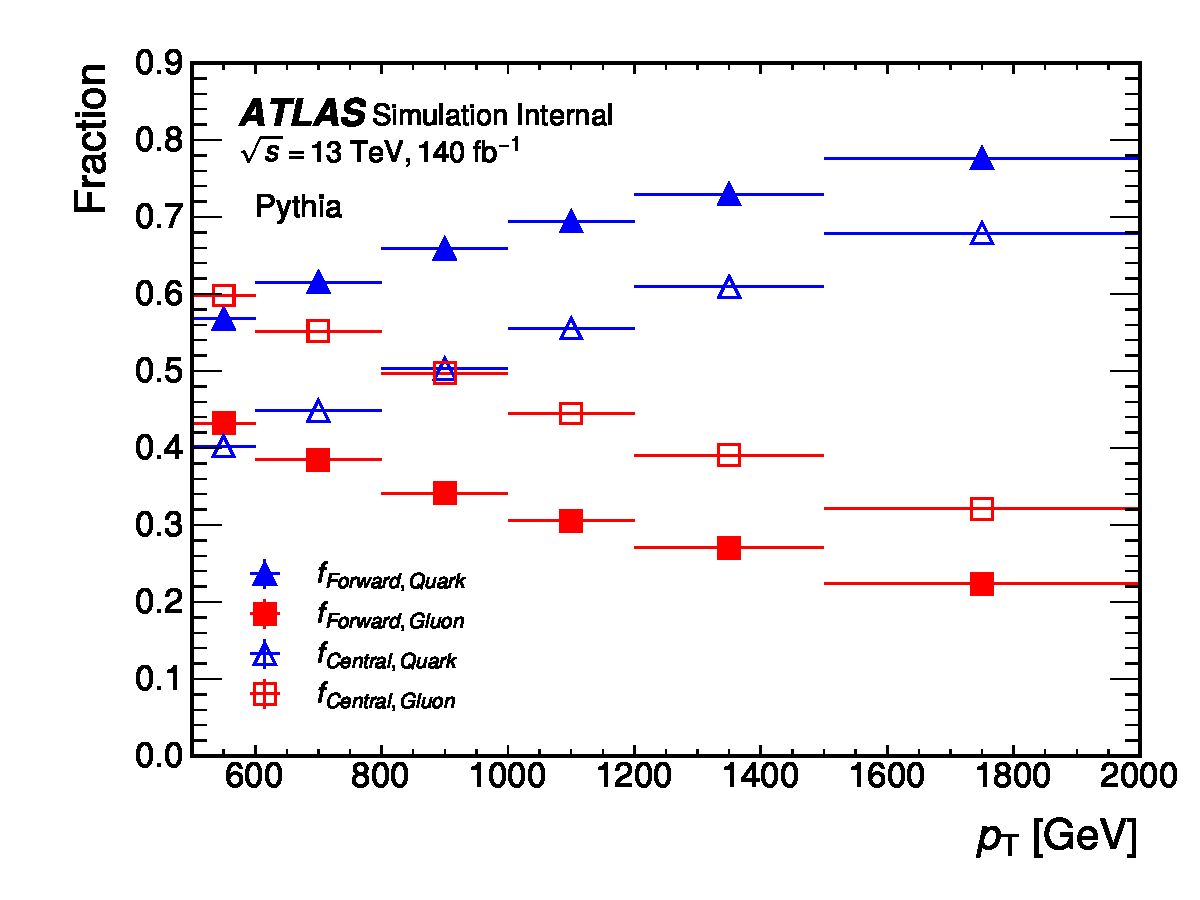
\includegraphics[width=0.6\textwidth]{fig/ADE/frac/Fraction_jet_nTracks_pythia.pdf}}\quad
	\caption[]{
		Fractions of quark-jets and gluon-jets  %
		in forward jet and central jet regions from {\pythia} dijet process. These values are used as elements in $F$ matrix in Equation \ref{eq:QG-matrix2}. %
		\label{fig:QG-Fmc}
	}
\end{figure}
%
%\begin{figure}[htb]
%	\centering
%	\subfloat[Forward region ]{\label{fig:QG-Quark-Fraction-forward}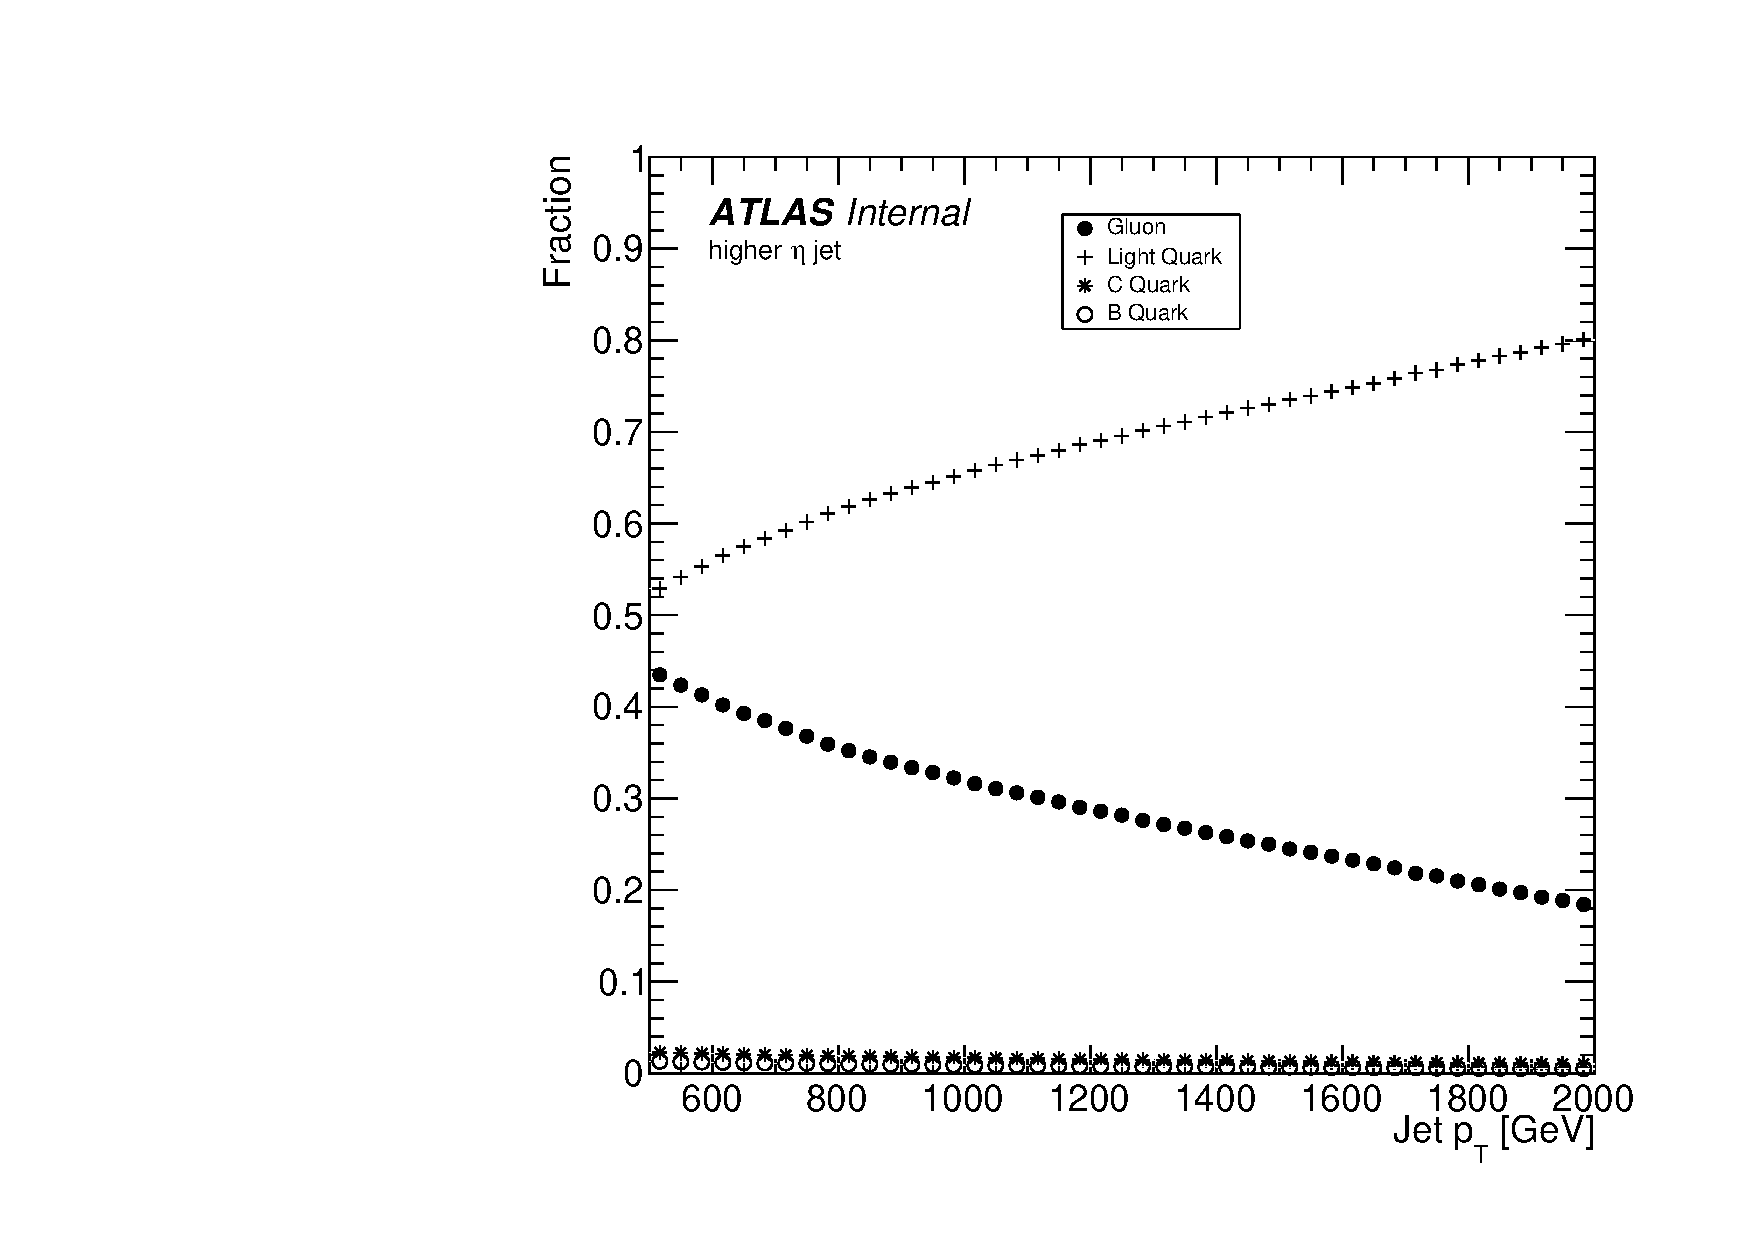
\includegraphics[width=0.45\textwidth]{fig/ADE/higher_fraction.pdf}} \quad
%	\subfloat[Central region ]{\label{fig:QG-Quark-Fraction-central}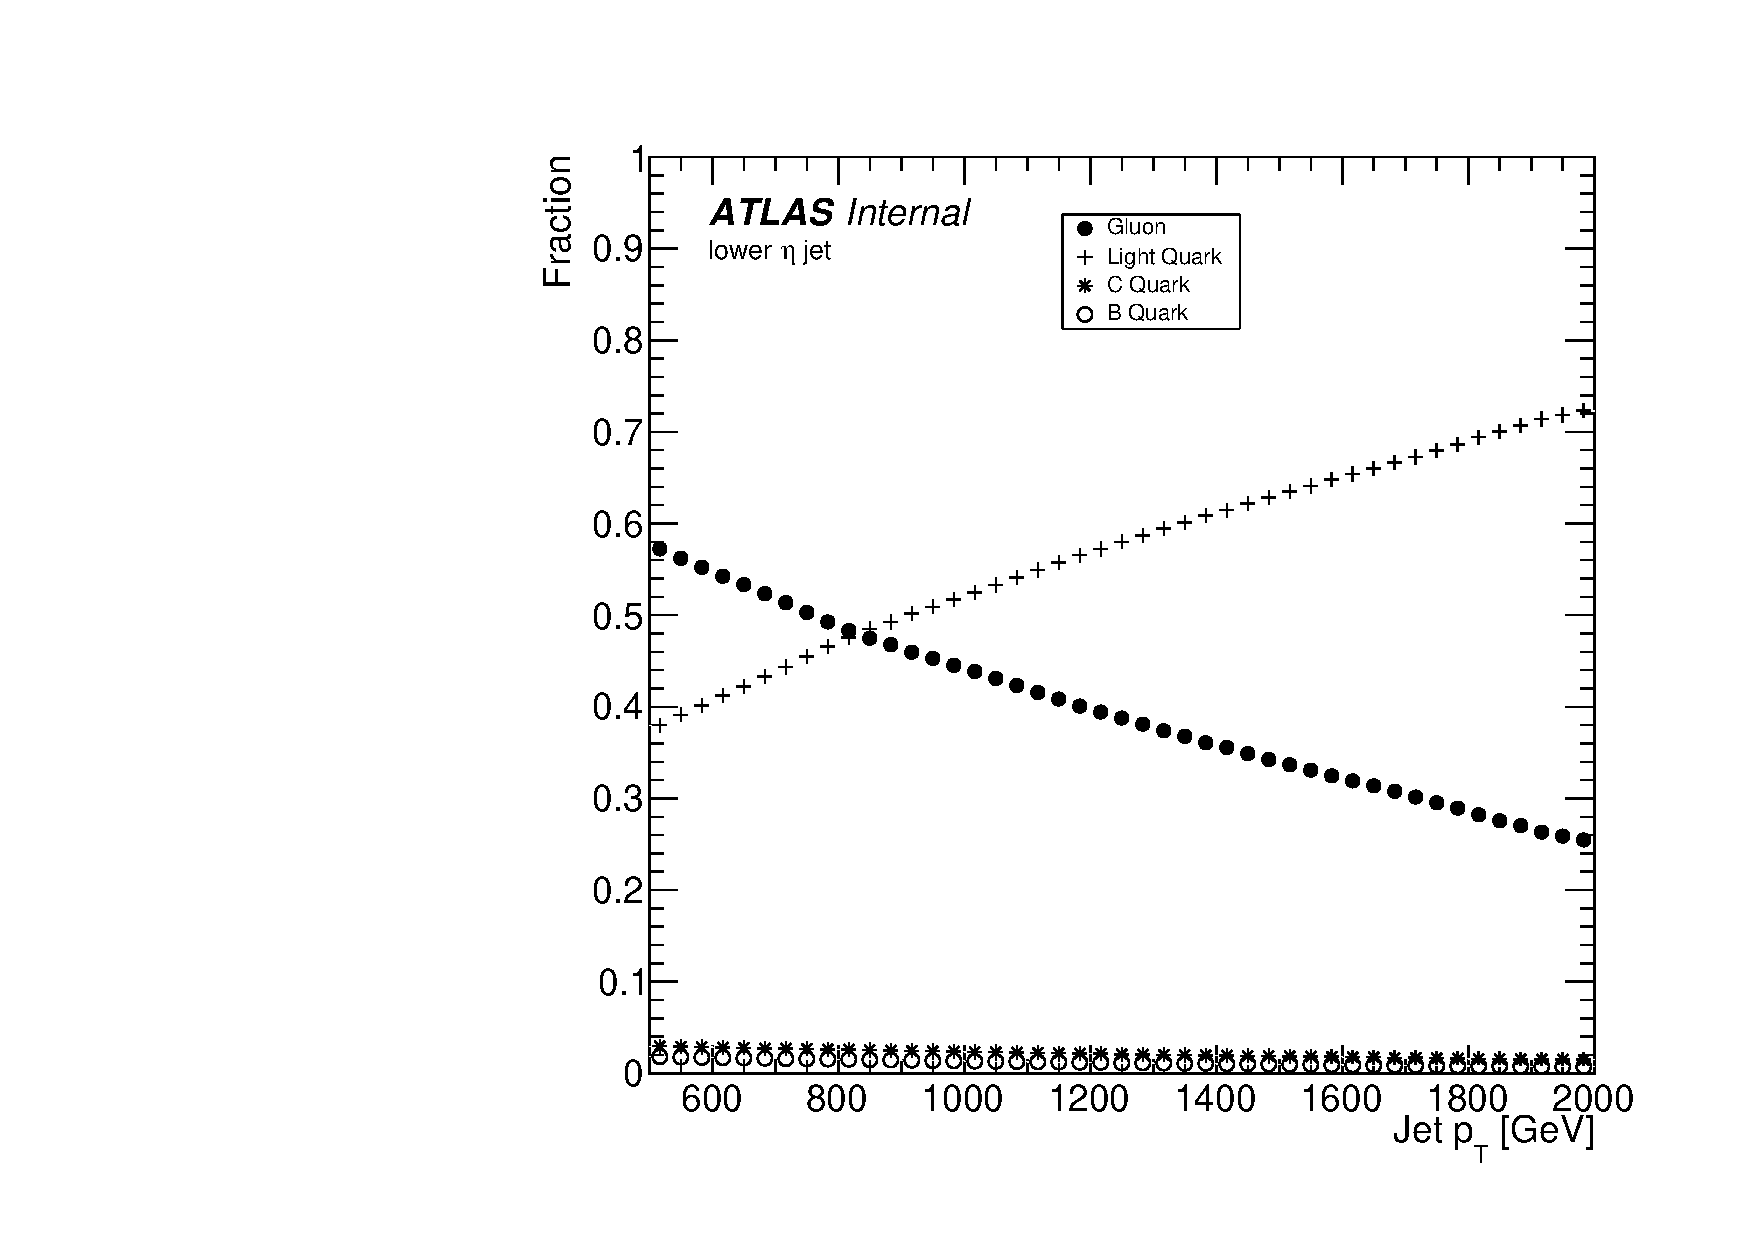
\includegraphics[width=0.45\textwidth]{fig/ADE/lower_fraction.pdf}} \quad
%	\caption[]{
%		Flavor composition of of forward \subref{fig:QG-Quark-Fraction-forward}  or central  \subref{fig:QG-Quark-Fraction-central} multi-jet events. %.
%		\label{fig:QG-quark-fraction}
%	}
%\end{figure}


%Figure~\ref{fig:QG-quark-fraction} illustrates the fraction of light and heavy quark- and gluon-jets in the \pythia8 dijet sample. These fractions are depicted in a stacked format, summing up to a cumulative value of 1. It should be noted that the involvement of heavy flavour quarks constitutes a minor fraction, amounting to a few percent, and is deemed negligible for the later study.
%Previous investigations have established that any discrepancies among the fractions derived from various MC event generators remain minimal. Furthermore, the shapes of distributions obtained from the MC simulations generally exhibit congruence with those observed within the  data.
%The distributions of \ntrk~and BDT score in higher and lower jet regions are shown in Figure~\ref{fig:QG-ntrk-method1} and Figure~\ref{fig:QG-jetHLPt} in jet \pt~range 500 GeV - 600 GeV. The shapes of distributions obtained from the MC simulations is generally consistent with that from data.
%
%\begin{figure}[htb]
%	\centering
%	\subfloat[Forward region]{\label{fig:QG-jetHLPta}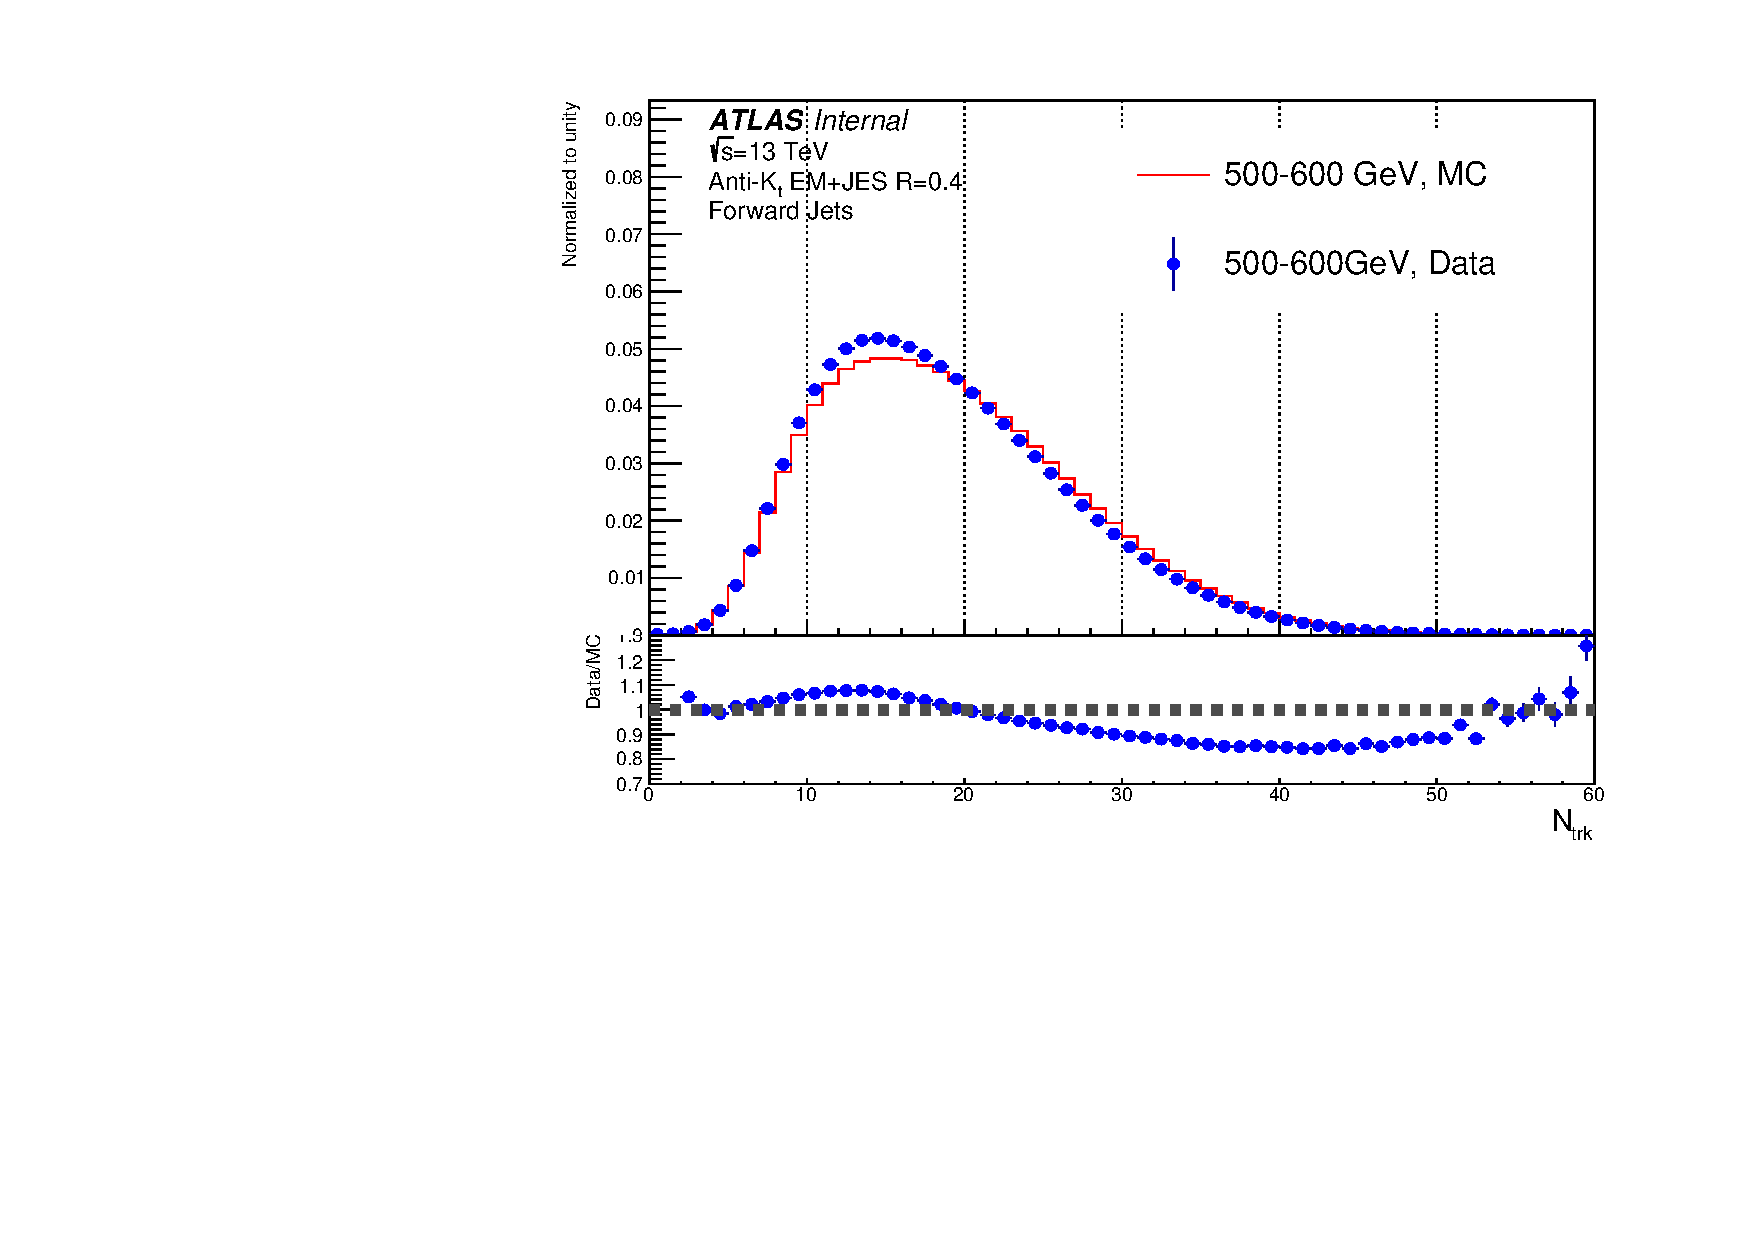
\includegraphics[width=0.45\textwidth]{fig/dijetanalysis/pythia-nominal/kinematics/ntrk_Forward_500_600_Pythia.pdf}} \quad
%	\subfloat[Central region ]{\label{fig:QG-jetHLPtb}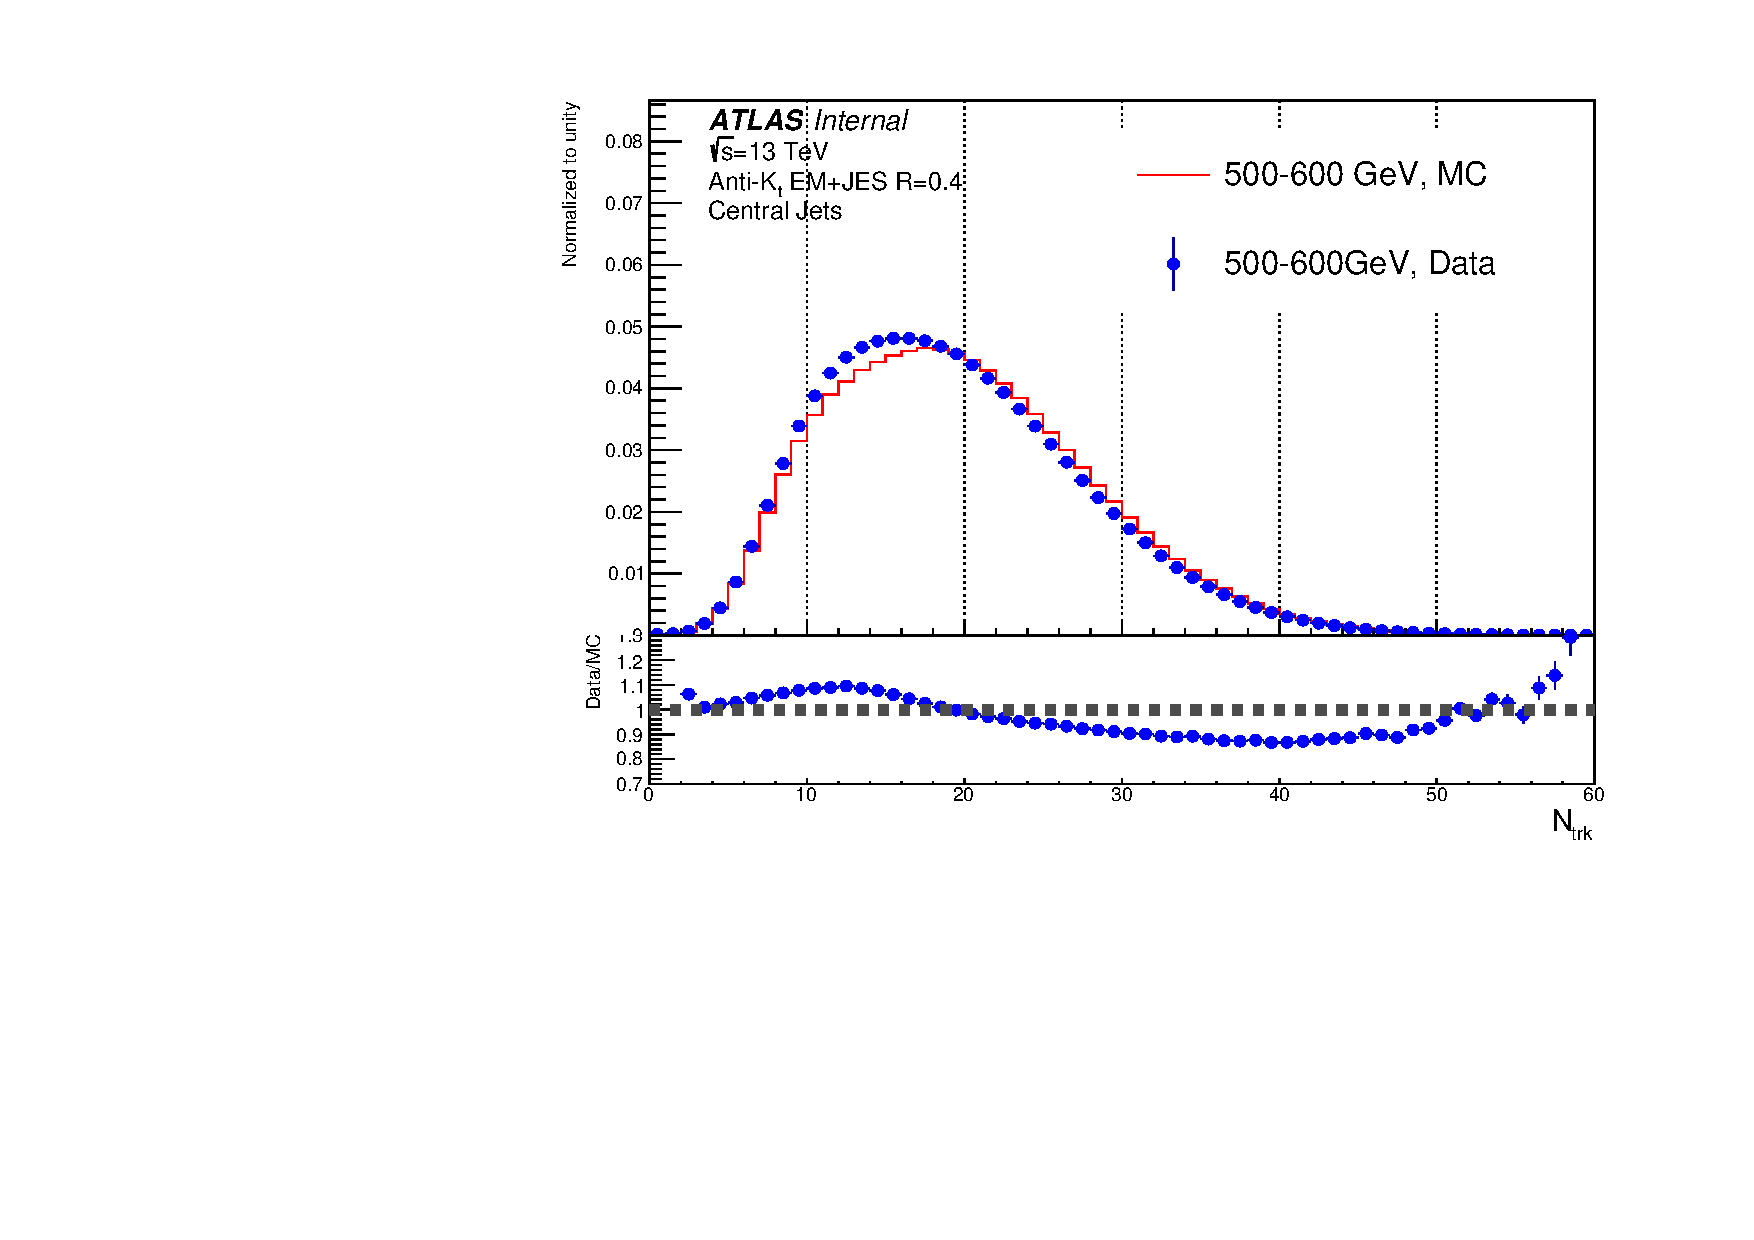
\includegraphics[width=0.45\textwidth]{fig/dijetanalysis/pythia-nominal/kinematics/ntrk_Central_500_600_Pythia.pdf}}\\
%	\caption[]{
%	  The \ntrk~distribution of the leading two jets with {\pythia8} in the MC and data.
%		\label{fig:QG-ntrk-method1}
%	}
%\end{figure}
%
%\begin{figure}[htb]
%	\centering
%	\subfloat[Forward region]{\label{fig:QG-jetHLPta}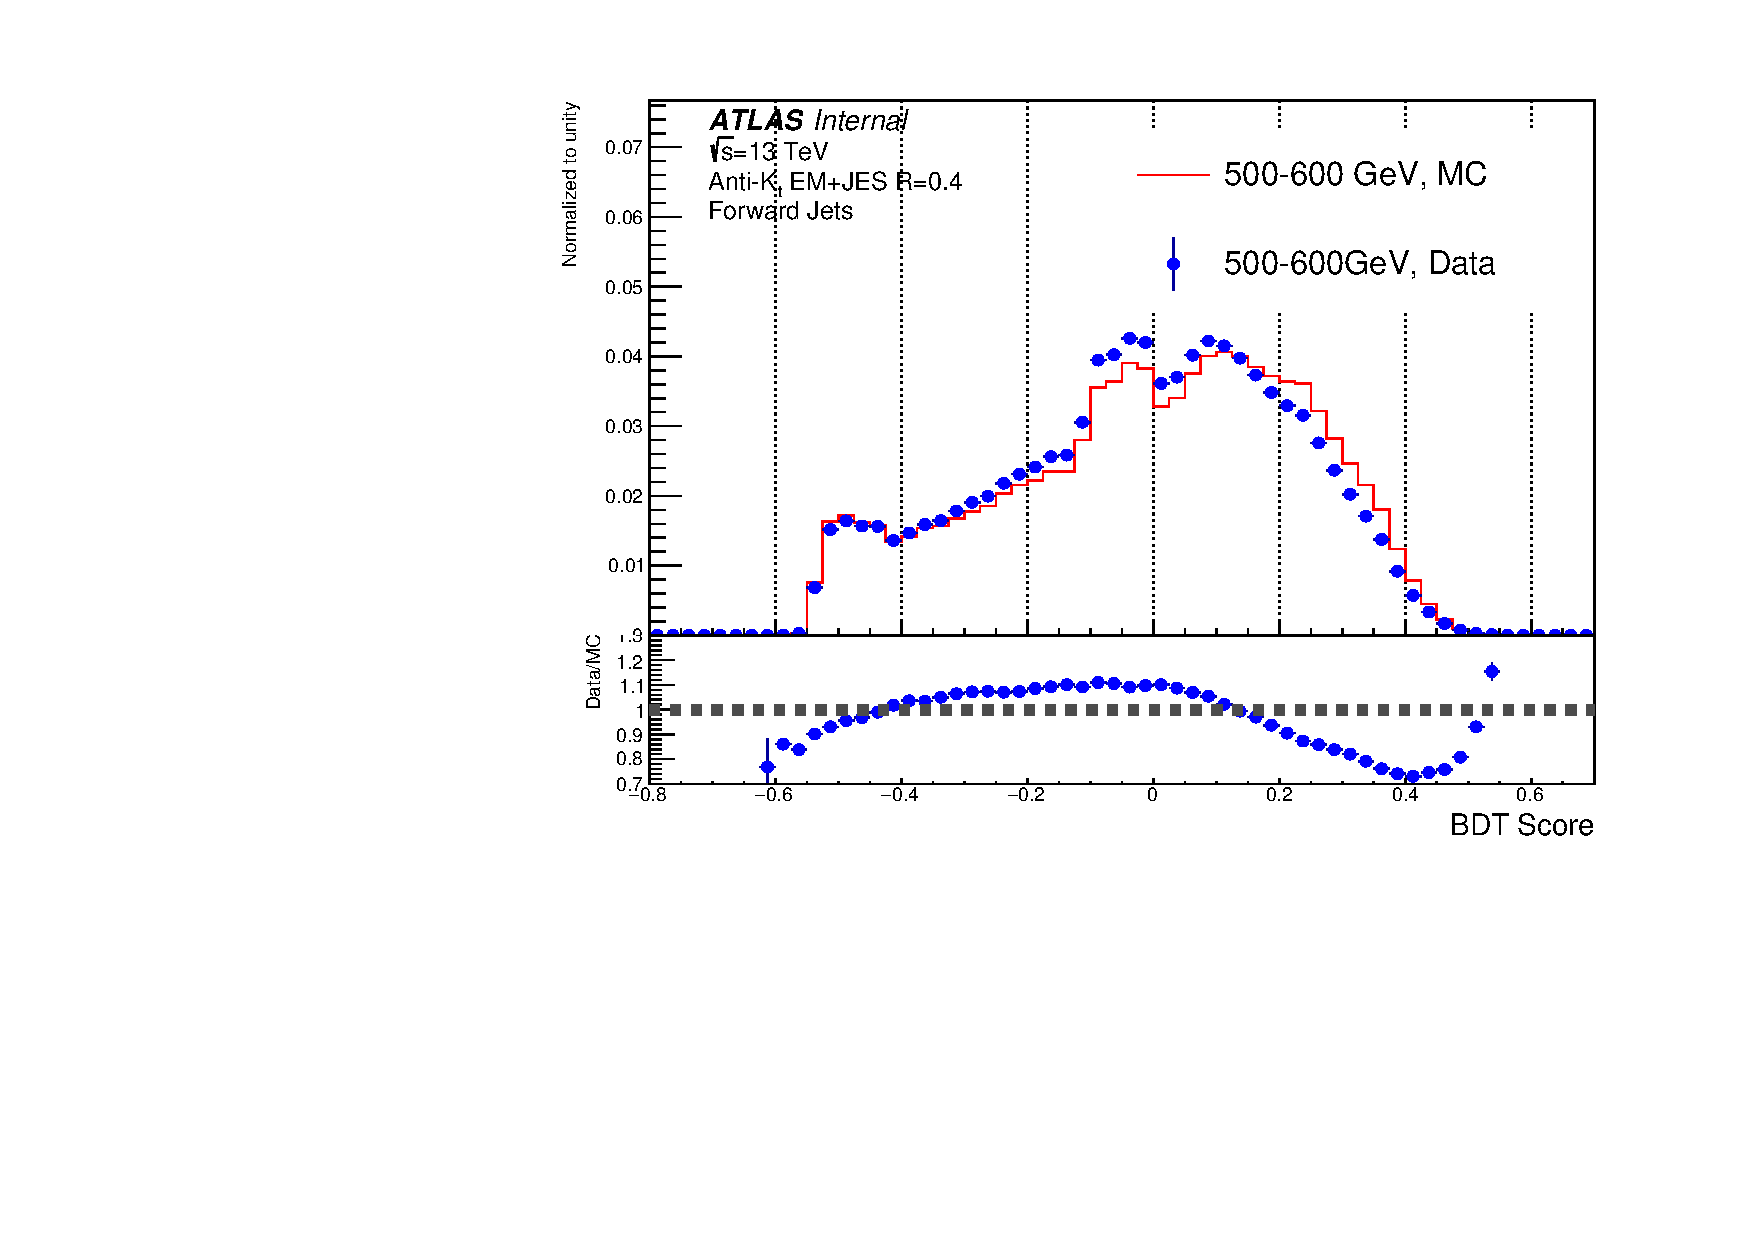
\includegraphics[width=0.45\textwidth]{fig/dijetanalysis/pythia-nominal/kinematics/bdt_Forward_500_600_Pythia.pdf}} \quad
%	\subfloat[Central region ]{\label{fig:QG-jetHLPtb}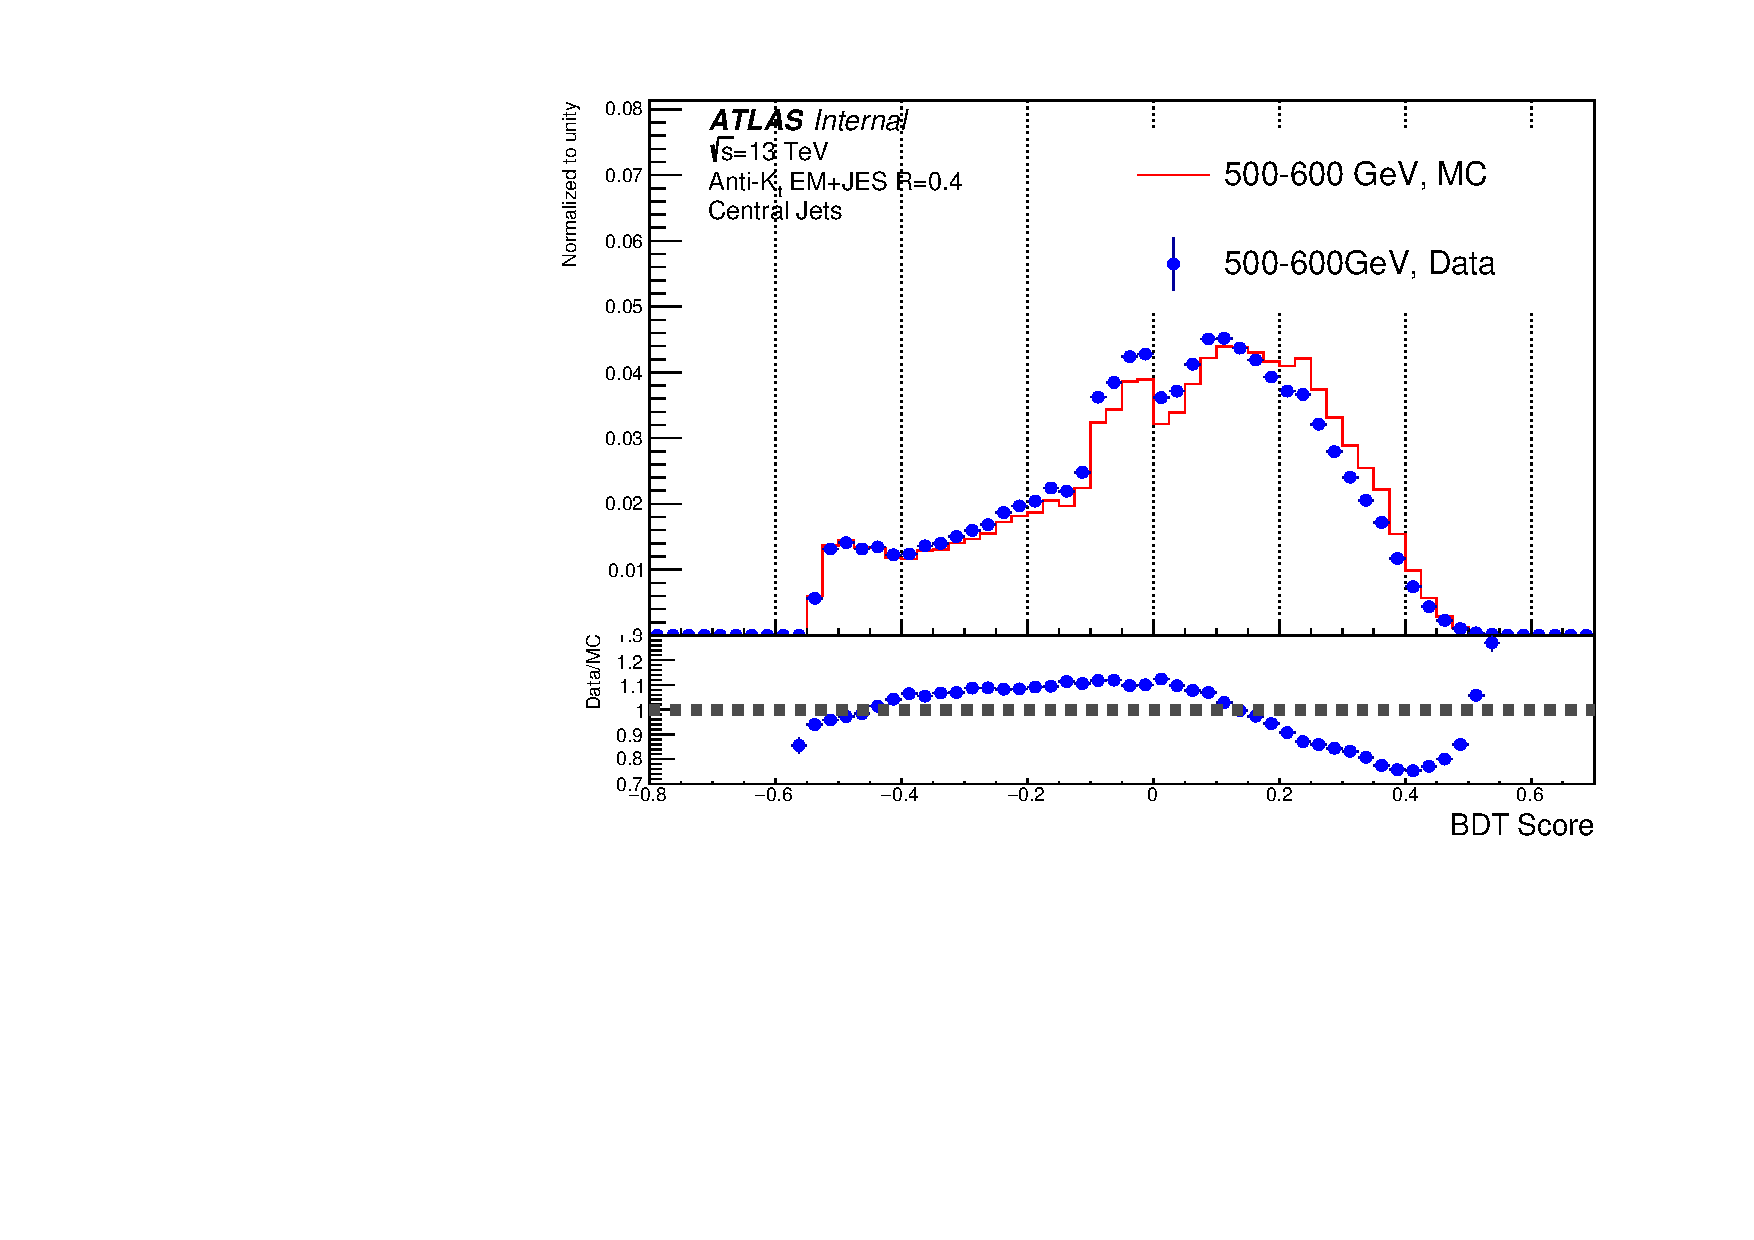
\includegraphics[width=0.45\textwidth]{fig/dijetanalysis/pythia-nominal/kinematics/bdt_Central_500_600_Pythia.pdf}}\\
%	\caption[]{
%	  The BDT score distribution of the leading two jets with {\pythia8} in the MC and data.
%	    %Data for four plots are 139\ifb in total.	The normalization of the simulation is decided by cross-section.
%		\label{fig:QG-jetHLPt}
%	}
%\end{figure}



%The matrix in 2-process extraction is given as 
%\begin{eqnarray}
%\label{eq:QG-matrix}
%\left(\begin{array}{c} 
%p_{\mrm{$\gamma$+jets}}(x)\\ 
%p_{\mrm{Multi-jet}}(x)\\ 
%\end{array}\right)
%&=&
%\underbrace{
%	\left(\begin{array}{cc}
%	f_{\mrm{$\gamma$+jets,Q}}&f_{\mrm{$\gamma$+jets,G}}\\
%	f_{\mrm{Multi-jet,Q}}&f_{\mrm{Multi-jet,G}}\\
%	\end{array}\right)
%}_{\scalebox{1}{$\equiv F$}}
%\left(\begin{array}{c} 
%p_\mrm{Q}(x)\\ 
%p_\mrm{G}(x)\\ 
%\end{array}\right)
%\\
%\label{eq:QG-invmatrix}
%\Leftrightarrow
%\left(\begin{array}{c} 
%p_\mrm{Q}(x)\\ 
%p_\mrm{G}(x)\\ 
%\end{array}\right)
%&=& F^{-1}
%\left(\begin{array}{c} 
%p_{\mrm{$\gamma$+jets}}(x)\\ 
%p_{\mrm{Multi-jet}}(x)\\ 
%\end{array}\right),
%\end{eqnarray}




%To estimate the systematic uncertainty coming from the parton shower modeling, %
%this calibration is performed for \pythia8 and \sherpa~separately. %
%%For \pythia8, both of the $Z$+jets and multi-jet MCs are \pythia8. %
%%For \sherpa, the $Z$+jets MC is \sherpa2.2.1 and the multi-jet MC is \sherpa2.1.1. %
%%This difference will be taken into account in the systematic uncertainties. %
%In \Sectrange{sec:QG-method}{sec:QG-SF}, the figures using \pythia8~(\sherpa) show results %
%with  NNPDF30~(NNPDF30) and NNPDF23LO~(CT10) PDF sets for 2-process extraction and for higher/lower \abseta jet extraction, respectively. %

%In \Sectrange{sec:QG-var}{sec:QG-SF}, the figures show the result with the \pythia8 parton shower modeling
%and the NNPDF30 PDF set for 2-process extraction or NNPDF23LO set for higher/lower \abseta jet. %
%A14 tuned NNPDF23LO set. %




%\begin{tabular}{l|l|c|c|cc}
% \hline
% \multicolumn{2}{l|}{\multirow{3}{*}{Selection}}& \multirow{3}{*}{$\gamma$+jets sample} & \multicolumn{3}{c}{Multi-jet sample}  \\ 
% \hhline{~~~---}
% \multicolumn{2}{l|}{} &                        & For 2-process & Higher |\etaX| & Lower |\etaX| \\ 
% \multicolumn{2}{l|}{} &                        & extraction    & jet sample  & jet sample \\ \hline 
% & Trigger   & Single photon trigger & \multicolumn{3}{c}{Or of single jet triggers} \\ 
% & MC-specialized cut & - & \multicolumn{3}{c}{$0.5<p_{\mrm{T,avg}}(\mrm{jets})/p_{\mrm{T,truth}}(j_1)<1.5$} \\ 
% & Number of jets        &  $\geq1$ & \multicolumn{3}{c}{$\geq2$} \\ \hhline{~~~---}
%  & $\pt$($\gamma$)             & $>125$     &-   & \multicolumn{2}{c}{-}   \\ 
% & $\pt(j_1)$             & $>50$     &$>50$  &\multicolumn{2}{c}{$>500$} \\ 
%  & $\pt(j_1)/\pt(j_2)$   &  -       & -    & \multicolumn{2}{c}{$<1.5$} \\ 
% & $|\eta(j_1)|$         &  $<2.1$  & $<2.1$ & \multicolumn{2}{c}{$<2.1$}   \\ 
% & $|\eta(j_2)|$         &  -       & -      & \multicolumn{2}{c}{$<2.1$}   \\ \hline
% & Target parton         &  Quark   & Gluon  & Quark  & Gluon       \\ \hhline{~-----}
% & Used jet in $j_1$ or $j_2$ & Only $j_1$ & Only $j_1$ & Higher $|\etaX|$ jet & Lower $|\etaX|$ jet \\
% \hline
%\end{tabular}

%In a low \pt range~($<500\GeV$), the quark fraction of  $\gamma$+jets is high~($\sim75\%$) %
%and the difference between the quark fractions in  $\gamma$+jets and multi-jet is large~($30$--$50\%$), %
%but the quark fraction of higher \abseta jet is low~($\lesssim 50\%$). % 
%Thus, the $\gamma$+jets and multi-jet are used as quark/gluon-enriched samples in the low \pt range. %
%In a high \pt range~($>500\GeVX$), higher \abseta jet has a large fraction of quarks~($>60\%$). %
%Thus, in the low \pt range, the higher/lower \abseta jet samples are used\footnote{
%The low statistics of $\gamma$+jets sample in the higher \pt range is another reason to use the higher/lower \abseta jet samples. %
%}. %
%The fractions are obtained from \pythia8 and \sherpa, separately. %


%\subsection{Method 1 for high \pt jet}
%\label{sec:method1_intro}

%\subsubsection{Background study}
%{\textcolor{red}{Wanyun: please add the background study here and tell people the background for dijet is negiligible}}
%In the whole \pt range, b-quark jets and jets labeled "other" exist, but it is suppressed to be lower than a few \%, which can be ignored. The jets labeled "other" are jets mainly originating from pileup.


%\FloatBarrier

% Data v.s. MC comparison in inclusive gamma+jets or Multi-jet(2sample ext.)

%\begin{figure}[htb]
%	\centering
%	\subfloat[$100<\pt<150\GeV$~(\sherpa) ]{\label{fig:QG-NtrkDataMCinclSherpaa}\includegraphics[width=0.45\textwidth]{Figures/dijetgammajetanalysis/MC_Closure/dist_comparison_plots/100-150_dist_total_comparison_ntrk_sherpa}} \quad
%	\subfloat[$500<\pt<600\GeV$~(\sherpa)]{\label{fig:QG-NtrkDataMCinclSherpab}\includegraphics[width=0.45\textwidth]{Figures/dijetgammajetanalysis/MC_Closure/dist_comparison_plots/500-600_dist_total_comparison_ntrk_sherpa}}\\
%	\subfloat[$100<\pt<150\GeV$~(\pythia8) ]{\label{fig:QG-WtrkDataMCincla}\includegraphics[width=0.45\textwidth]{Figures/dijetgammajetanalysis/MC_Closure/dist_comparison_plots/100-150_dist_total_comparison_ntrk_pythia}} \quad
%	\subfloat[$500<\pt<600\GeV$~(\pythia8)]{\label{fig:QG-WtrkDataMCinclb}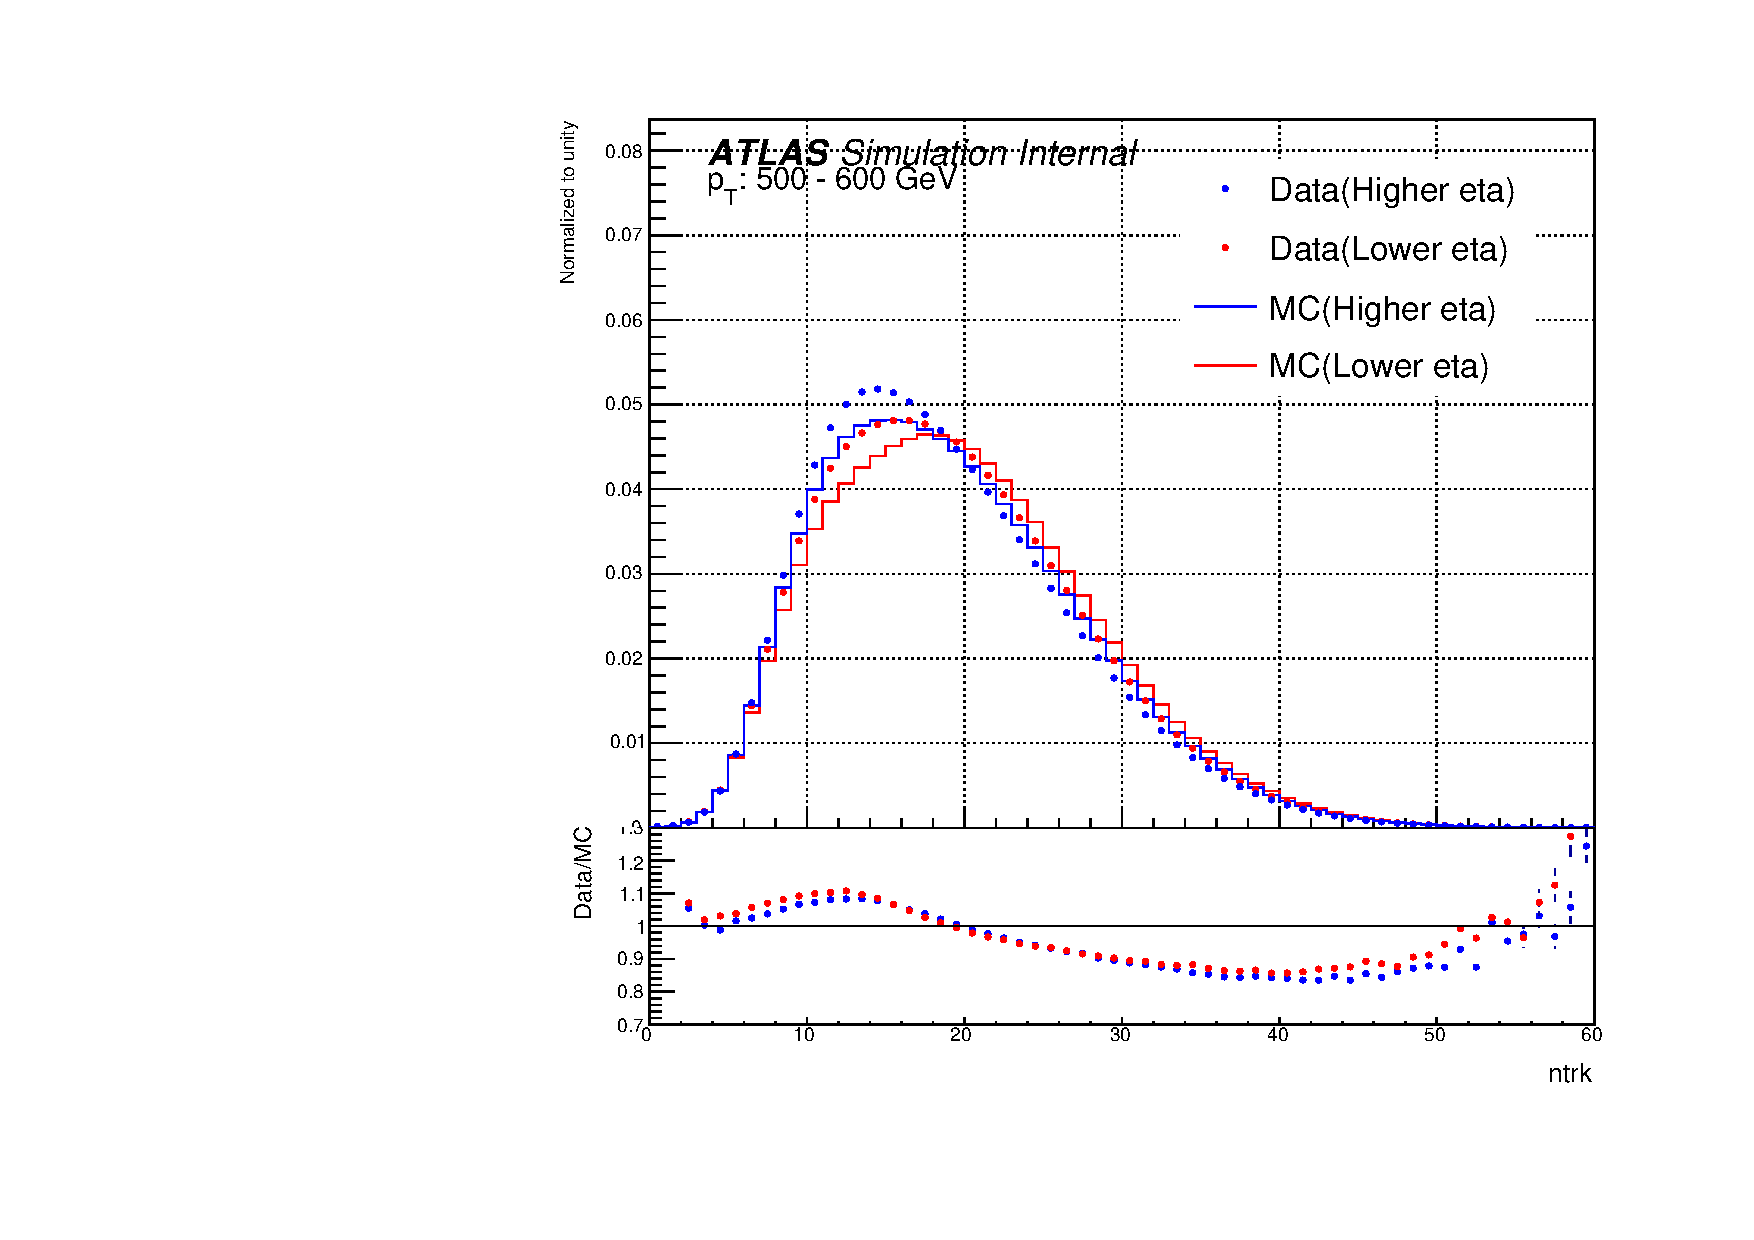
\includegraphics[width=0.45\textwidth]{Figures/dijetgammajetanalysis/MC_Closure/dist_comparison_plots/500-600_dist_total_comparison_ntrk_pythia}}
%	\caption[]{
%		The comparison between the data and MC with \sherpa  \subref{fig:QG-NtrkDataMCinclSherpaa} 	\subref{fig:QG-NtrkDataMCinclSherpab} and \pythia \subref{fig:QG-WtrkDataMCincla}  \subref{fig:QG-WtrkDataMCinclb} in \ntrk distributions of $\gamma$+jets and multi-jet events used in 2-sample extraction. %
%		Graphs and solid-line histograms show the \ntrk distributions in the data and MC, respectively.
%		Bottom panels show the ratio of the data to the MC in each of $\gamma$+jets and multi-jet events. %
%		\label{fig:QG-NtrkDataMCinclSherpa}
%	}
%\end{figure}
%
%\begin{figure}[htb]
%	\centering
%	\subfloat[$500<\pt<600\GeV$~(\sherpa) ]{\label{fig:QG-BDTDataMCinclSherpaa11}\includegraphics[width=0.45\textwidth]{Figures/dijetanalysis/higher-lower-sf/sherpa_MC_500_ntrk}} \quad
%	\subfloat[$800<\pt<1000\GeV$~(\sherpa)]{\label{fig:QG-BDTDataMCinclSherpab12}\includegraphics[width=0.45\textwidth]{Figures/dijetanalysis/higher-lower-sf/sherpa_MC_800_ntrk}}\\
%	\subfloat[$500<\pt<600\GeV$~(\pythia8) ]{\label{fig:QG-BDTDataMCinclPythiaa31}\includegraphics[width=0.45\textwidth]{Figures/dijetanalysis/higher-lower-sf/pythia_MC_500_ntrk}} \quad
%	\subfloat[$800<\pt<1000\GeV$~(\pythia8)]{\label{fig:QG-BDTDataMCinclPythiab41}\includegraphics[width=0.45\textwidth]{Figures/dijetanalysis/higher-lower-sf/pythia_MC_800_ntrk}}
%	\caption[]{
%		The comparison between the data and MC with \sherpa \subref{fig:QG-BDTDataMCinclSherpaa11} \subref{fig:QG-BDTDataMCinclSherpab21} and \pythia \subref{fig:QG-BDTDataMCinclPythiaa31} \subref{fig:QG-BDTDataMCinclPythiab41} in \nrtk distributions of higher or lower $\abseta$ multi-jet events used in 2-process extraction. %
%		Graphs and solid-line histograms show the \nrtk distributions in the data and MC, respectively.
%		Bottom panels show the ratio of the data to the MC in each of $\gamma$+jets and multi-jet events. %
%		\label{fig:QG-BDTDataMCinclPythia1}
%	}
%\end{figure}



%\begin{figure}[htb]
%	\centering
%	\subfloat[$50<\pt<600\GeV$~(\sherpa) ]{\label{fig:QG-WtrkDataMCinclaaa}\includegraphics[width=0.45\textwidth]{Figures/dijetanalysis/higher-lower-sf/sherpa_MC_500_ntrk}} \quad
%	\subfloat[$800<\pt<1000\GeV$~(\sherpa)]{\label{fig:QG-WtrkDataMCinclbbb}\includegraphics[width=0.45\textwidth]{Figures/dijetanalysis/higher-lower-sf/sherpa_MC_800_ntrk}}\\
%	\subfloat[$50<\pt<600\GeV$~(\pythia8) ]{\label{fig:QG-WtrkDataMCincla}\includegraphics[width=0.45\textwidth]{Figures/dijetanalysis/higher-lower-sf/pythia_MC_500_ntrk}} \quad
%	\subfloat[$800<\pt<1000\GeV$~(\pythia8)]{\label{fig:QG-WtrkDataMCinclb}\includegraphics[width=0.45\textwidth]{Figures/dijetanalysis/higher-lower-sf/pythia_MC_800_ntrk}}
%	\caption[]{
%		The comparison between the data and MC with \sherpa\subref{fig:QG-WtrkDataMCinclaaa} \subref{fig:QG-WtrkDataMCinclbbb} and \pythia \subref{fig:QG-WtrkDataMCincla} \subref{fig:QG-WtrkDataMCinclb} in \ntrk distributions of higher or lower $\abseta$ multi-jet events in 2-process extraction. %
%		Graphs and solid-line histograms show the \ntrk distributions in the data and MC, respectively.
%		Bottom panels show the ratio of the data to the MC in each of $\gamma$+jets and multi-jet events. %
%		\label{fig:QG-NtrkDataMCinclPythia}
%	}
%\end{figure}
%
%
%\begin{figure}[htb]
%	\centering
%	\subfloat[$100<\pt<150\GeV$~(\sherpa) ]{\label{fig:QG-WtrkDataMCinclSherpaa}\includegraphics[width=0.45\textwidth]{Figures/dijetgammajetanalysis/MC_Closure/dist_comparison_plots/100-150_dist_total_comparison_width_sherpa}} \quad
%	\subfloat[$500<\pt<600\GeV$~(\sherpa)]{\label{fig:QG-WtrkDataMCinclSherpab}\includegraphics[width=0.45\textwidth]{Figures/dijetgammajetanalysis/MC_Closure/dist_comparison_plots/500-600_dist_total_comparison_width_sherpa}}
%	\caption[]{
%		The comparison between the data and MC in \wtrk distributions of $\gamma$+jets and multi-jet events used in 2-sample extraction %
%		in \subref{fig:QG-WtrkDataMCinclSherpaa} the jet \pt range from 100 to 150\GeV and %
%		\subref{fig:QG-WtrkDataMCinclSherpab} from 500 to 600\GeV. %
%		Graphs and solid-line histograms show the \wtrk distributions in the data and MC, respectively.
%		Bottom panels show the ratio of the data to the MC in each of $\gamma$+jets and multi-jet events. %
%		\label{fig:QG-WtrkDataMCinclSherpa}
%	}
%\end{figure}
%
%\begin{figure}[htb]
%	\centering
%	\subfloat[$100<\pt<150\GeV$~(\pythia) ]{\label{fig:QG-WtrkDataMCinclSherpaa1}\includegraphics[width=0.45\textwidth]{Figures/dijetgammajetanalysis/MC_Closure/dist_comparison_plots/100-150_dist_total_comparison_width_pythia}} \quad
%	\subfloat[$500<\pt<600\GeV$~(\pythia)]{\label{fig:QG-WtrkDataMCinclSherpab1}\includegraphics[width=0.45\textwidth]{Figures/dijetgammajetanalysis/MC_Closure/dist_comparison_plots/500-600_dist_total_comparison_width_pythia}}
%	\caption[]{
%		The comparison between the data and MC in \wtrk distributions of $\gamma$+jets and multi-jet events used in 2-sample extraction %
%		in \subref{fig:QG-WtrkDataMCinclSherpaa} the jet \pt range from 100 to 150\GeV and %
%		\subref{fig:QG-WtrkDataMCinclSherpab} from 500 to 600\GeV. %
%		Graphs and solid-line histograms show the \wtrk distributions in the data and MC, respectively.
%		Bottom panels show the ratio of the data to the MC in each of $\gamma$+jets and multi-jet events. %
%		\label{fig:QG-WtrkDataMCinclSherpa1}
%	}
%\end{figure}
%
%\begin{figure}[htb]
%	\centering
%	\subfloat[$100<\pt<150\GeV$~(\sherpa) ]{\label{fig:QG-C1B02DataMCinclSherpaa}\includegraphics[width=0.45\textwidth]{Figures/dijetgammajetanalysis/MC_Closure/dist_comparison_plots/100-150_dist_total_comparison_c1_pythia}} \quad
%	\subfloat[$500<\pt<600\GeV$~(\sherpa)]{\label{fig:QG-C1B02DataMCinclSherpab}\includegraphics[width=0.45\textwidth]{Figures/dijetgammajetanalysis/MC_Closure/dist_comparison_plots/500-600_dist_total_comparison_c1_sherpa}}
%	\caption[]{
%		The comparison between the data and MC in \cbeta distributions of $\gamma$+jets and multi-jet events used in 2-sample extraction %
%		in \subref{fig:QG-C1B02DataMCinclSherpaa} the jet \pt range from 100 to 150\GeV and %
%		\subref{fig:QG-C1B02DataMCinclSherpab} from 500 to 600\GeV. %
%		Graphs and solid-line histograms show the \cbeta distributions in the data and MC, respectively.
%		Bottom panels show the ratio of the data to the MC in each of $\gamma$+jets and multi-jet events. %
%		\label{fig:QG-C1B02DataMCinclSherpa}
%	}
%\end{figure}
%
%\begin{figure}[htb]
%	\centering
%	\subfloat[$100<\pt<150\GeV$~(\pythia8) ]{\label{fig:QG-C1B02DataMCinclPythiaa}\includegraphics[width=0.45\textwidth]{Figures/dijetgammajetanalysis/MC_Closure/dist_comparison_plots/100-150_dist_total_comparison_c1_pythia}} \quad
%	\subfloat[$500<\pt<600\GeV$~(\pythia8)]{\label{fig:QG-C1B02DataMCinclPythiab}\includegraphics[width=0.45\textwidth]{Figures/dijetgammajetanalysis/MC_Closure/dist_comparison_plots/500-600_dist_total_comparison_c1_pythia}}
%	\caption[]{
%		The comparison between the data and MC in \cbeta distributions of $\gamma$ +jets and multi-jet events used in 2-sample extraction %
%		in \subref{fig:QG-C1B02DataMCinclPythiaa} the jet \pt range from 100 to 150\GeV and %
%		\subref{fig:QG-C1B02DataMCinclPythiab} from 500 to 600\GeV. %
%		Graphs and solid-line histograms show the \cbeta distributions in the data and MC, respectively.
%		Bottom panels show the ratio of the data to the MC in each of $\gamma$+jets and multi-jet events. %
%		\label{fig:QG-C1B02DataMCinclPythia}
%	}
%\end{figure}


%\begin{figure}[htb]
%	\centering
%	\subfloat[$100<\pt<150\GeV$~(\sherpa) ]{\label{fig:QG-BDTDataMCinclSherpaa}\includegraphics[width=0.45\textwidth]{Figures/dijetgammajetanalysis/MC_Closure/dist_comparison_plots/100-150_dist_total_comparison_bdt_sherpa}} \quad
%	\subfloat[$500<\pt<600\GeV$~(\sherpa)]{\label{fig:QG-BDTDataMCinclSherpab}\includegraphics[width=0.45\textwidth]{Figures/dijetgammajetanalysis/MC_Closure/dist_comparison_plots/500-600_dist_total_comparison_bdt_sherpa}}\\
%	\subfloat[$100<\pt<150\GeV$~(\pythia8) ]{\label{fig:QG-BDTDataMCinclPythiaa}\includegraphics[width=0.45\textwidth]{Figures/dijetgammajetanalysis/MC_Closure/dist_comparison_plots/100-150_dist_total_comparison_bdt_pythia}} \quad
%	\subfloat[$500<\pt<600\GeV$~(\pythia8)]{\label{fig:QG-BDTDataMCinclPythiab}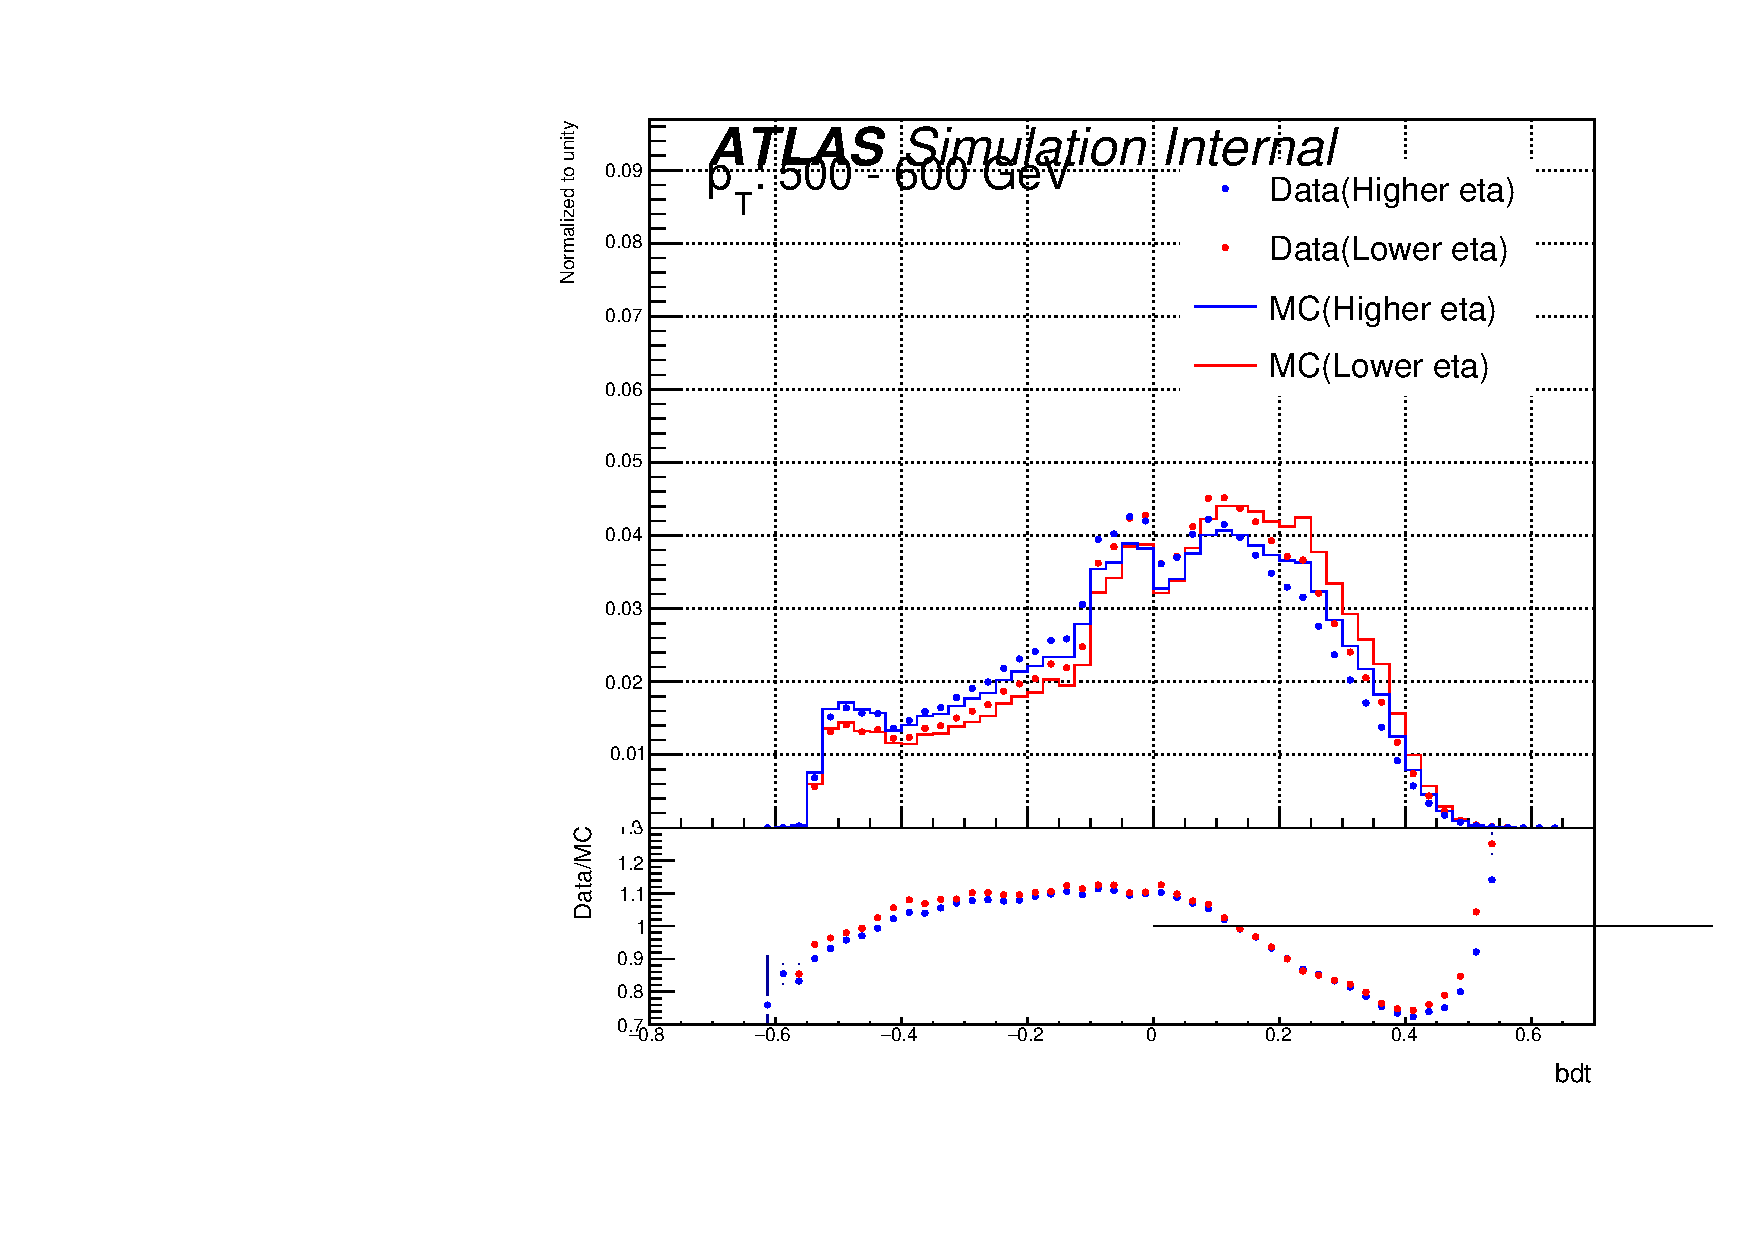
\includegraphics[width=0.45\textwidth]{Figures/dijetgammajetanalysis/MC_Closure/dist_comparison_plots/500-600_dist_total_comparison_bdt_pythia}}
%	\caption[]{
%		The comparison between the data and MC with \sherpa \subref{fig:QG-BDTDataMCinclSherpaa} \subref{fig:QG-BDTDataMCinclSherpab} and \pythia \subref{fig:QG-BDTDataMCinclPythiaa} \subref{fig:QG-BDTDataMCinclPythiab}  in BDT distributions of $\gamma$+jets and multi-jet events used in 2-sample extraction.V. %
%		Graphs and solid-line histograms show the BDT distributions in the data and MC, respectively.
%		Bottom panels show the ratio of the data to the MC in each of $\gamma$+jets and multi-jet events. %
%		\label{fig:QG-BDTDataMCinclSherpa}
%	}
%\end{figure}
%\begin{figure}[htb]
%	\centering
%\subfloat[$500<\pt<600\GeV$~(\sherpa) ]{\label{fig:QG-BDTDataMCinclSherpaa1}\includegraphics[width=0.45\textwidth]{Figures/dijetanalysis/higher-lower-sf/sherpa_MC_500_bdt}} \quad
%\subfloat[$800<\pt<1000\GeV$~(\sherpa)]{\label{fig:QG-BDTDataMCinclSherpab2}\includegraphics[width=0.45\textwidth]{Figures/dijetanalysis/higher-lower-sf/sherpa_MC_800_bdt}}\\
%\subfloat[$500<\pt<600\GeV$~(\pythia8) ]{\label{fig:QG-BDTDataMCinclPythiaa3}\includegraphics[width=0.45\textwidth]{Figures/dijetanalysis/higher-lower-sf/pythia_MC_500_bdt}} \quad
%\subfloat[$800<\pt<1000\GeV$~(\pythia8)]{\label{fig:QG-BDTDataMCinclPythiab4}\includegraphics[width=0.45\textwidth]{Figures/dijetanalysis/higher-lower-sf/pythia_MC_800_bdt}}
%	\caption[]{
%		The comparison between the data and MC with \sherpa \subref{fig:QG-BDTDataMCinclSherpaa1} \subref{fig:QG-BDTDataMCinclSherpab2} and \pythia \subref{fig:QG-BDTDataMCinclPythiaa3} \subref{fig:QG-BDTDataMCinclPythiab4} in BDT distributions of higher or lower $\abseta$ multi-jet events used in 2-process extraction. %
%		Graphs and solid-line histograms show the BDT distributions in the data and MC, respectively.
%		Bottom panels show the ratio of the data to the MC in each of $\gamma$+jets and multi-jet events. %
%		\label{fig:QG-BDTDataMCinclPythia}
%	}
%\end{figure}

%\subsection{Method 2 for low \pt jet}
%\label{sec:method2_intro}
%\subsubsection{Prescale trigger}
%{\textcolor{red}{Wanyun and Rongqian: please add the study of prescale here for low pt dijet events}}
%The ATLAS trigger system consists of a hardware-based component, the Level-1 (L1), a software-based trigger system, the higher-level trigger (HLT) or Event Filter (EF). The HLT runs a simplified version of the ATLAS reconstruction software. On the HLT-level calibrated jets defined by the anti-kt algorithm with R = 0.4 are used. The calibration is close to the one of off-line jets. In this note the performance is evaluated with respect to PFlow jets.
%Each trigger item uses a L1 trigger and a HLT trigger. The L1 system first evaluates for each given trigger if it is passed. To keep the trigger rate at an acceptable level, the triggers with high trigger rate are only read-out for a fraction of all events ("prescales”). The prescale is a number applied on-line by the ATLAS trigger system. If an event passes the conditions set by the trigger system, the prescale for the L1 trigger and for the HLT trigger is decided. If the L1 or the HLT trigger is prescaled the HLT trigger decision is not evaluated in order to save computing time. The prescales for the L1 trigger and the HLT trigger are decided independently.
%The composition of the triggers used here is summarized in \Tab{tab:prescaletrigger}
%The jet \pT spectra for each of the triggers are shown in .{\textcolor{red}{Rongqian: please link jet triggers spectrum (before unprescaling) here}}\ref{fig:QG-b-ps}
%
%\begin{figure}[htb]
%	\centering
%	\subfloat[2017]{\label{fig:QG-2017ps}\includegraphics[width=0.45\textwidth]{Figures/Method2/Triggers/data17_single_trigger_Inclusive.pdf}}\quad
%	\subfloat[2018]{\label{fig:QG-2018ps}\includegraphics[width=0.45\textwidth]{Figures/Method2/Triggers/data18_single_trigger_Inclusive.pdf}}
%	\caption[]{
%	  The spectra for each jet trigger before unprescaling \subref{fig:QG-2017ps} is the 2017 dataset and \subref{fig:QG-b-ps} is the 2018 dataset.%
%		\label{fig:QG-b-ps}
%	}
%\end{figure}
%
%The jet \pT spectra can be corrected by the average prescale calculated by the ratio of luminosity collected by a given trigger and the total luminosity. The values in \href{https://aiatlas046.cern.ch/tagservices/RunBrowser/runBrowserReport/runBrowserReport.php?fnt=data18_13TeV&pn=*&cn=*}{COMA trigger report}are used. The corrected jet \pT spectra for each trigger are shown{\textcolor{red}{Rongqian: please link jet triggers spectrum (after unprescaling) here}}\ref{fig:QG-a-ps}
%
%\begin{figure}[htb]
%	\centering
%	\subfloat[2017]{\label{fig:QG-2017ps}\includegraphics[width=0.45\textwidth]{Figures/Method2/Triggers/data17single_trigger_InclusivePS.pdf}}\quad
%	\subfloat[2018]{\label{fig:QG-2018ps}\includegraphics[width=0.45\textwidth]{Figures/Method2/Triggers/data18single_trigger_InclusivePS.pdf}}
%	\caption[]{
%	  The spectra for each jet trigger after unprescaling \subref{fig:QG-2017ps} is the 2017 dataset and \subref{fig:QG-2018ps} is the 2018 dataset.%
%		\label{fig:QG-a-ps}
%	}
%\end{figure}
%
%\begin{table}[htb]
%	\centering
%	\caption{
%		The summary of the prescale HLT triggers used in this calibration. %
%	}
%	\begin{tabular}{c}
%		\whline
%		Trigger name \\
%		\hline
%		 HLT\_j35 \\
%		  HLT\_j45 \\
%		  HLT\_j60 \\
%		  HLT\_j110 \\
%		  HLT\_j175 \\
%		  HLT\_j260 \\
%		  HLT\_j360 \\
%		  \hline
%	 \end{tabular}
%	\label{tab:prescaletrigger}
%\end{table}
%
%
%
%{\textcolor{red}{Rongqian: please make the same plot in above section (method 1) for method 2 and put them here. Please put the plots in 100-150 and 400-500 GeV bins here and put others in appendix. }
%
%\begin{figure}[htb]
%	\centering
%	\subfloat[For $\gamma$+jets and multi-jet extraction~(\sherpa) ]{\label{fig:QG-Fmcc}\includegraphics[width=0.45\textwidth]{Figures/Method2/fraction/pt-fraction_pt.pdf}}\quad
%	\subfloat[For $\gamma$+jets and multi-jet extraction~(\pythia) ]{\label{fig:QG-Fmcd}\includegraphics[width=0.45\textwidth]{Figures/placeholder}}
%	\caption[]{
%	  (\textcolor{red}{Rongqian}) Fractions of quark jets and gluon jets in each of \subref{fig:QG-Fmcc} \subref{fig:QG-Fmcd} SHERPA and PYTHIA $\gamma$+jets and multi-jet for 2-process extraction %
%		$\gamma$+jets and multi-jets  %
%		These values are used as elements in $F$ matrix in \Eqn{eq:QG-matrix}(\ref{eq:QG-invmatrix}). %
%		\label{fig:QG-Fmc}
%	}
%\end{figure}
%
%
%\begin{figure}[htb]
%	\centering
%	\subfloat[$\gamma$+jets~(\sherpa)]{\label{fig:QG-jetMethod2Pta}\includegraphics[width=0.45\textwidth]{Figures/Method2/Pt-spectrum/GammaJet_Sherpa_pt_distribution.pdf}} \quad
%	\subfloat[multi-jet ~(\sherpa) ]{\label{fig:QG-jetHLPtb}\includegraphics[width=0.45\textwidth]{Figures/Method2/Pt-spectrum/LeadingJet_Dijet_Inclusive.png}}\\
%	\subfloat[$\gamma$+jets~(\pythia)]{\label{fig:QG-jetMethod2Ptaa}\includegraphics[width=0.45\textwidth]{Figures/placeholder}} \quad
%	\subfloat[multi-jet ~(\pythia) ]{\label{fig:QG-jetMethod2Ptbb}\includegraphics[width=0.45\textwidth]{Figures/placeholder}}
%%	\subfloat[$\gamma$+jets~(\sherpa)]{\label{fig:QG-jetMethod2Pta}\includegraphics[width=0.45\textwidth]{Figures/newplot/sherpa_higher_pt}} \quad
%%	\subfloat[multi-jet ~(\sherpa) ]{\label{fig:QG-jetMethod2Ptb}\includegraphics[width=0.45\textwidth]{Figures/newplot/sherpa_lower_pt}}\\
%%	\subfloat[$\gamma$+jets~(\pythia)]{\label{fig:QG-jetMethod2Ptaa}\includegraphics[width=0.45\textwidth]{Figures/dijetanalysis/pt-spectrum/powpyt_higher_pt}} \quad
%%	\subfloat[multi-jet ~(\pythia) ]{\label{fig:QG-jetMethod2Ptbb}\includegraphics[width=0.45\textwidth]{Figures/dijetanalysis/pt-spectrum/powpyt_lower_pt}}
%	\caption[]{
%	  (\textcolor{red}{Rongqian})The \pt distribution of the leading jets with \sherpa  \subref{fig:QG-jetMethod2Pta}  \subref{fig:QG-jetMethod2Ptb}  and \pythia 
%		 \subref{fig:QG-jetMethod2Ptaa}  \subref{fig:QG-jetMethod2Ptbb}  in  \subref{fig:QG-jetMethod2Pta} the $\gamma$+jets   %
%		and \subref{fig:QG-jetMethod2Ptb} the multi-jet extraction.
%	    %Data for four plots are 139\ifb in total.	The normalization of the simulation is decided by cross-section.
%		\label{fig:QG-jetMethod2Pt}
%	}
%\end{figure}
%
%\begin{figure}[htb]
%	\centering
%	\subfloat[$\gamma$+jets~(\sherpa)]{\label{fig:QG-jetHLPta}\includegraphics[width=0.45\textwidth]{Figures/Method2/kinematics/Gammajet-eta.png}} \quad
%	\subfloat[multi-jet~(\sherpa) ]{\label{fig:QG-jetHLPtb}\includegraphics[width=0.45\textwidth]{Figures/Method2/kinematics/Dijet_Sherpa_eta.png}}\\
%	\subfloat[$\gamma$+jets~(\pythia)]{\label{fig:QG-jetHLPtaa}\includegraphics[width=0.45\textwidth]{Figures/placeholder}} \quad
%	\subfloat[multi-jet~(\pythia) ]{\label{fig:QG-jetHLPtbb}\includegraphics[width=0.45\textwidth]{Figures/placeholder}}
%%	\subfloat[$\gamma$+jets~(\sherpa)]{\label{fig:QG-jetHLPta}\includegraphics[width=0.45\textwidth]{Figures/newplot/sherpa_higher_pt}} \quad
%%	\subfloat[Lower \abseta jet~(\sherpa) ]{\label{fig:QG-jetHLPtb}\includegraphics[width=0.45\textwidth]{Figures/newplot/sherpa_lower_pt}}\\
%%	\subfloat[Higher \abseta jet~(\pythia)]{\label{fig:QG-jetHLPtaa}\includegraphics[width=0.45\textwidth]{Figures/dijetanalysis/pt-spectrum/powpyt_higher_pt}} \quad
%%	\subfloat[Lower \abseta jet~(\pythia) ]{\label{fig:QG-jetHLPtbb}\includegraphics[width=0.45\textwidth]{Figures/dijetanalysis/pt-spectrum/powpyt_lower_pt}}
%	\caption[]{
%	  (\textcolor{red}{Rongqian})The \eta distribution of the jets with \sherpa  \subref{fig:QG-jetHLPta}  \subref{fig:QG-jetHLPtb}  and \pythia 
%		 \subref{fig:QG-jetHLPtaa}  \subref{fig:QG-jetHLPtbb}  in  \subref{fig:QG-jetHLPta} the $\gamma$+jets   %
%		and \subref{fig:QG-jetHLPtb} the multi-jet extraction.
%	    %Data for four plots are 139\ifb in total.	The normalization of the simulation is decided by cross-section.
%		\label{fig:QG-eta-method1}
%	}
%\end{figure}
%
%\begin{figure}[htb]
%	\centering
%	\subfloat[$\gamma$+jets~(\sherpa)]{\label{fig:QG-jetHLPta}\includegraphics[width=0.45\textwidth]{Figures/Method2/kinematics/Gammajet-ntrk.png}} \quad
%	\subfloat[multi-jet~(\sherpa) ]{\label{fig:QG-jetHLPtb}\includegraphics[width=0.45\textwidth]{Figures/Method2/kinematics/Dijet_Sherpa_ntrk.png}}\\
%	\subfloat[$\gamma$+jets~(\pythia)]{\label{fig:QG-jetHLPtaa}\includegraphics[width=0.45\textwidth]{Figures/placeholder}} \quad
%	\subfloat[multi-jet~(\pythia) ]{\label{fig:QG-jetHLPtbb}\includegraphics[width=0.45\textwidth]{Figures/placeholder}}
%%	\subfloat[Higher \abseta jet~(\sherpa)]{\label{fig:QG-jetHLPta}\includegraphics[width=0.45\textwidth]{Figures/newplot/sherpa_higher_pt}} \quad
%%	\subfloat[Lower \abseta jet~(\sherpa) ]{\label{fig:QG-jetHLPtb}\includegraphics[width=0.45\textwidth]{Figures/newplot/sherpa_lower_pt}}\\
%%	\subfloat[Higher \abseta jet~(\pythia)]{\label{fig:QG-jetHLPtaa}\includegraphics[width=0.45\textwidth]{Figures/dijetanalysis/pt-spectrum/powpyt_higher_pt}} \quad
%%	\subfloat[Lower \abseta jet~(\pythia) ]{\label{fig:QG-jetHLPtbb}\includegraphics[width=0.45\textwidth]{Figures/dijetanalysis/pt-spectrum/powpyt_lower_pt}}
%	\caption[]{
%	  (\textcolor{red}{Rongqian})The \ntrk distribution of the jets with \sherpa  \subref{fig:QG-jetHLPta}  \subref{fig:QG-jetHLPtb}  and \pythia 
%		 \subref{fig:QG-jetHLPtaa}  \subref{fig:QG-jetHLPtbb}  in  \subref{fig:QG-jetHLPta} the $\gamma$+jets   %
%		and \subref{fig:QG-jetHLPtb} the multi-jet extraction.
%	    %Data for four plots are 139\ifb in total.	The normalization of the simulation is decided by cross-section.
%		\label{fig:QG-ntrk-method1}
%	}
%\end{figure}
%
%\begin{figure}[htb]
%	\centering
%	\subfloat[$\gamma$+jets~(\sherpa)]{\label{fig:QG-jetHLPta}\includegraphics[width=0.45\textwidth]{Figures/Method2/kinematics/Gammajet-width.png}} \quad
%	\subfloat[multi-jet~(\sherpa) ]{\label{fig:QG-jetHLPtb}\includegraphics[width=0.45\textwidth]{Figures/Method2/kinematics/Dijet_Sherpa_width.png}}\\
%	\subfloat[$\gamma$+jets~(\pythia)]{\label{fig:QG-jetHLPtaa}\includegraphics[width=0.45\textwidth]{Figures/placeholder}} \quad
%	\subfloat[multi-jet~(\pythia) ]{\label{fig:QG-jetHLPtbb}\includegraphics[width=0.45\textwidth]{Figures/placeholder}}
%%	\subfloat[Higher \abseta jet~(\sherpa)]{\label{fig:QG-jetHLPta}\includegraphics[width=0.45\textwidth]{Figures/newplot/sherpa_higher_pt}} \quad
%%	\subfloat[Lower \abseta jet~(\sherpa) ]{\label{fig:QG-jetHLPtb}\includegraphics[width=0.45\textwidth]{Figures/newplot/sherpa_lower_pt}}\\
%%	\subfloat[Higher \abseta jet~(\pythia)]{\label{fig:QG-jetHLPtaa}\includegraphics[width=0.45\textwidth]{Figures/dijetanalysis/pt-spectrum/powpyt_higher_pt}} \quad
%%	\subfloat[Lower \abseta jet~(\pythia) ]{\label{fig:QG-jetHLPtbb}\includegraphics[width=0.45\textwidth]{Figures/dijetanalysis/pt-spectrum/powpyt_lower_pt}}
%	\caption[]{
%	  (\textcolor{red}{Rongqian})The \wtrk distribution of the leading jets with \sherpa  \subref{fig:QG-jetHLPta}  \subref{fig:QG-jetHLPtb}  and \pythia 
%		 \subref{fig:QG-jetHLPtaa}  \subref{fig:QG-jetHLPtbb}  in  \subref{fig:QG-jetHLPta} the $\gamma$+jets   %
%		and \subref{fig:QG-jetHLPtb} the multi-jet extraction.
%	    %Data for four plots are 139\ifb in total.	The normalization of the simulation is decided by cross-section.
%		\label{fig:QG-wtrk-methed1}
%	}
%\end{figure}
%
%\begin{figure}[htb]
%	\centering
%	\subfloat[$\gamma$+jets~(\sherpa)]{\label{fig:QG-jetHLPta}\includegraphics[width=0.45\textwidth]{Figures/Method2/kinematics/Gammajet-c1.png}} \quad
%	\subfloat[multi-jet~(\sherpa) ]{\label{fig:QG-jetHLPtb}\includegraphics[width=0.45\textwidth]{Figures/Method2/kinematics/Dijet_Sherpa_c1.png}}\\
%	\subfloat[$\gamma$+jets~(\pythia)]{\label{fig:QG-jetHLPtaa}\includegraphics[width=0.45\textwidth]{Figures/placeholder}} \quad
%	\subfloat[multi-jet jet~(\pythia) ]{\label{fig:QG-jetHLPtbb}\includegraphics[width=0.45\textwidth]{Figures/placeholder}}
%%	\subfloat[Higher \abseta jet~(\sherpa)]{\label{fig:QG-jetHLPta}\includegraphics[width=0.45\textwidth]{Figures/newplot/sherpa_higher_pt}} \quad
%%	\subfloat[Lower \abseta jet~(\sherpa) ]{\label{fig:QG-jetHLPtb}\includegraphics[width=0.45\textwidth]{Figures/newplot/sherpa_lower_pt}}\\
%%	\subfloat[Higher \abseta jet~(\pythia)]{\label{fig:QG-jetHLPtaa}\includegraphics[width=0.45\textwidth]{Figures/dijetanalysis/pt-spectrum/powpyt_higher_pt}} \quad
%%	\subfloat[Lower \abseta jet~(\pythia) ]{\label{fig:QG-jetHLPtbb}\includegraphics[width=0.45\textwidth]{Figures/dijetanalysis/pt-spectrum/powpyt_lower_pt}}
%	\caption[]{
%	  (\textcolor{red}{Rongqian})The C1 distribution of the jets with \sherpa  \subref{fig:QG-jetHLPta}  \subref{fig:QG-jetHLPtb}  and \pythia 
%		 \subref{fig:QG-jetHLPtaa}  \subref{fig:QG-jetHLPtbb}  in  \subref{fig:QG-jetHLPta} the $\gamma$+jets   %
%		and \subref{fig:QG-jetHLPtb} the multi-jet extraction.
%	    %Data for four plots are 139\ifb in total.	The normalization of the simulation is decided by cross-section.
%		\label{fig:QG-wtrk-methed1}
%	}
%\end{figure}
%
%\begin{figure}[htb]
%	\centering
%	\subfloat[$100<\pt<150\GeV$~(\sherpa) ]{\label{fig:QG-NtrkDataMCinclSherpaa}\includegraphics[width=0.45\textwidth]{Figures/Method2/SF-MC/100-150_dist_total_comparison_ntrk_sherpa.pdf}} \quad
%	\subfloat[400<\pt<500\GeV$~(\sherpa)]{\label{fig:QG-NtrkDataMCinclSherpab}\includegraphics[width=0.45\textwidth]{Figures/Method2/SF-MC/400-500_dist_total_comparison_ntrk_sherpa.pdf}}\\
%	\subfloat[$100<\pt<150\GeV$~(\pythia8) ]{\label{fig:QG-WtrkDataMCincla}\includegraphics[width=0.45\textwidth]{Figures/Method2/SF-MC/}} \quad
%	\subfloat[$400<\pt<500\GeV$~(\pythia8)]{\label{fig:QG-WtrkDataMCinclb}\includegraphics[width=0.45\textwidth]{Figures/Method2/SF-MC/}}
%	\caption[]{
%		The comparison between the data and MC with \sherpa  \subref{fig:QG-NtrkDataMCinclSherpaa} 	\subref{fig:QG-NtrkDataMCinclSherpab} and \pythia \subref{fig:QG-WtrkDataMCincla}  \subref{fig:QG-WtrkDataMCinclb} in \ntrk distributions of $\gamma$+jets and multi-jet events used in 2-sample extraction. %
%		Graphs and solid-line histograms show the \ntrk distributions in the data and MC, respectively.
%		Bottom panels show the ratio of the data to the MC in each of $\gamma$+jets and multi-jet events. %
%		\label{fig:QG-NtrkDataMCinclSherpa}
%	}
%\end{figure}
%
%\begin{figure}[htb]
%	\centering
%	\subfloat[$100<\pt<150\GeV$~(\sherpa) ]{\label{fig:QG-NtrkDataMCinclSherpaa}\includegraphics[width=0.45\textwidth]{Figures/Method2/SF-MC/100-150_dist_total_comparison_bdt_sherpa.pdf}} \quad
%	\subfloat[400<\pt<500\GeV$~(\sherpa)]{\label{fig:QG-NtrkDataMCinclSherpab}\includegraphics[width=0.45\textwidth]{Figures/Method2/SF-MC/400-500_dist_total_comparison_bdt_sherpa.pdf}}\\
%	\subfloat[$100<\pt<150\GeV$~(\pythia8) ]{\label{fig:QG-WtrkDataMCincla}\includegraphics[width=0.45\textwidth]{Figures/Method2/SF-MC/}} \quad
%	\subfloat[$400<\pt<500\GeV$~(\pythia8)]{\label{fig:QG-WtrkDataMCinclb}\includegraphics[width=0.45\textwidth]{Figures/Method2/SF-MC/}}
%	\caption[]{
%		The comparison between the data and MC with \sherpa  \subref{fig:QG-NtrkDataMCinclSherpaa} 	\subref{fig:QG-NtrkDataMCinclSherpab} and \pythia \subref{fig:QG-WtrkDataMCincla}  \subref{fig:QG-WtrkDataMCinclb} in BDT distributions of $\gamma$+jets and multi-jet events used in 2-sample extraction. %
%		Graphs and solid-line histograms show the BDT distributions in the data and MC, respectively.
%		Bottom panels show the ratio of the data to the MC in each of $\gamma$+jets and multi-jet events. %
%		\label{fig:QG-NtrkDataMCinclSherpa}
%	}
%\end{figure}
%
%\begin{figure}[htb]
%	\centering
%	\subfloat[$100<\pt<150\GeV$~(\sherpa) ]{\label{fig:QG-BDT1}\includegraphics[width=0.45\textwidth]{Figures/Method2/roc/plots/roc-var/ROC_100-150_dijet.pdf}} \quad
%	\subfloat[400<\pt<500\GeV$~(\sherpa)]{\label{fig:QG-BDT2}\includegraphics[width=0.45\textwidth]{Figures/Method2/roc/plots/roc-var/ROC_400-500_dijet.pdf}}\\
%	\subfloat[$100<\pt<150\GeV$~(\pythia8) ]{\label{fig:QG-WtrkDataMCincla}\includegraphics[width=0.45\textwidth]{Figures/Method2/SF-MC/}} \quad
%	\subfloat[$400<\pt<500\GeV$~(\pythia8)]{\label{fig:QG-WtrkDataMCinclb}\includegraphics[width=0.45\textwidth]{Figures/Method2/SF-MC/}}
%	\caption[]{
%		ROC curve for different jet taggers%
%		\label{fig:QG-NtrkDataMCinclSherpa}
%	}
%\end{figure}
%
%
%\subsubsection{Background study}
%{\textcolor{red}{Wanyun and Rongqian: please add the background study here (ABCD) and tell people the background for dijet is negiligible}}
%
%
%
%\subsection{Validation} (\textcolor{red}{let's skip this section for now})
%\label{subsec:Validation }
%
%In addition to the primary samples defined above, several samples with very high quark or gluon-jet fractions are defined to validate the extracted templates in different topologies. The high purity is achieved by the use of event-level kinematic cuts. One is trijet sample used for validation of the extracted gluon template, Events are required to have a leading jet which passes the lowest unprescaled single jet trigger and a pT of at least 500 GeV. There must be at least two additional jets with \pT $>$ 20 GeV. All three jets must have $\abseta$ $<$ 2.1. The third jet is very likely to be gluon initiated in certain regions of phase space. The other one is $\gamma$+2jets sample, which has high quark-jet purity,The basic event selection is the same as for the $\gamma$+jet sample, with the exceptions that there should be at least one sub-leading jet with \pT > 20 GeV and $\abseta$ $<$ 2.1. 
\FloatBarrier
